% !TEX root = ../VanderbiltDissertationTemplate/dissertationOG.tex
% Chapter 5: CulinaryCut (ECCV 2026 main paper and supplementary material).
% Original ECCV figure filenames, including capitalization and spaces, are retained.
% This file is included from the dissertation main document; do not compile it alone.

\clearpage
\chapter{CulinaryCut: Physics-Grounded Cutting for Vision--Language--Action Models}
\label{CH5_CUTTINGSIM}

\noindent\textit{This chapter is adapted from \citet{koh2026culinarycut}, published in the proceedings of the European Conference on Computer Vision (ECCV 2026), with co-authors Hyunseo Koh, Youngjae Choi, Misa Viveiros, David Hyde, and Heewon Kim.}

% Consistent Chapter 5 table typography. The caption keeps the dissertation's style;
% the table body uses 9-pt type and single spacing without width-dependent scaling.
\providecommand{\CutTableSetup}{%
  \small
  \setstretch{1}%
  \setlength{\tabcolsep}{3.5pt}%
  \renewcommand{\arraystretch}{1.16}%
}

\section{Overview}
\label{sec:cut_overview}

Food cutting is a challenging deformable-object manipulation task: positioning the knife correctly does not guarantee separation. Successful execution must localize the target, overcome material-dependent contact resistance, and account for geometry and topology changes during cutting. A kinematically valid path can therefore fail when deformable-material dynamics are included.

This chapter presents \emph{CulinaryCut}, a physics-grounded benchmark generated with \emph{IntSim}, which couples a Moving Least Squares Material Point Method (MLS-MPM) material solver~\citep{2018-MLSMPM} to ManiSkill~\citep{gu2023ManiSkill2}. ManiSkill supplies robot execution and images; MLS-MPM computes deformation, tool contact, reaction forces, and cutting outcomes. Together, they evaluate physical separation rather than geometric blade motion alone.

Rather than introducing a new force-conditioned policy architecture, our objective is to study whether \emph{physics-grounded training data} improve existing vision--language--action (VLA) models. The benchmark separates two limitations:
\begin{itemize}
  \item \textbf{Geometry gap:} difficulty grounding language-specified ratios, directions, object identities, and sequential cuts in the actual geometry of a deformable object.
  \item \textbf{Physics gap:} difficulty producing sufficient material-dependent interaction to sever an object, even when the predicted knife path satisfies geometric criteria.
\end{itemize}
These gaps are related but distinct: a policy may select the correct cutting location without inducing a successful cut, or may produce a physically strong action at the wrong location.

CulinaryCut contains \textbf{21,000 physics-grounded cutting trajectories} spanning \textbf{15 food items}. Fifteen visual backgrounds and at least five instruction variants per trajectory expand the collection to approximately \textbf{1.575 million observation--instruction instances}. Contact-force profiles and material dynamics are retained in the generated data and used for simulation analysis and trajectory generation; \emph{force, contact, and damage states are not supplied as policy inputs}. We evaluate the existing RDT~\citep{liu2025rdt1bdiffusionfoundationmodel}, Octo~\citep{mees2024octo}, and OpenVLA~\citep{openvla} policies without changing their architectures. This distinction is important: the contribution is a physics-grounded dataset and evaluation protocol, not a closed-loop force-feedback controller or an additional style-transfer network.

\subsection{Research Motivation and Contributions}
\label{subsec:cut_motivation}

The main contributions are:
\begin{enumerate}
  \item \textbf{Physics-grounded simulation and benchmarking:} coupling robot execution with MLS-MPM deformation, damage, contact forces, and separation.
  \item \textbf{Geometry- and physics-gap analyses:} measuring ratio, direction, object, and sequential-cut generalization separately from material severing.
  \item \textbf{Scalable data generation:} constructing 21,000 trajectories for 15 foods and approximately 1.575 million visually and linguistically augmented instances.
  \item \textbf{Empirical validation:} comparing real and simulated contact forces and evaluating physics-grounded policy training in simulation and on a real robot.
\end{enumerate}

\begin{figure}[!htbp]
  \centering
  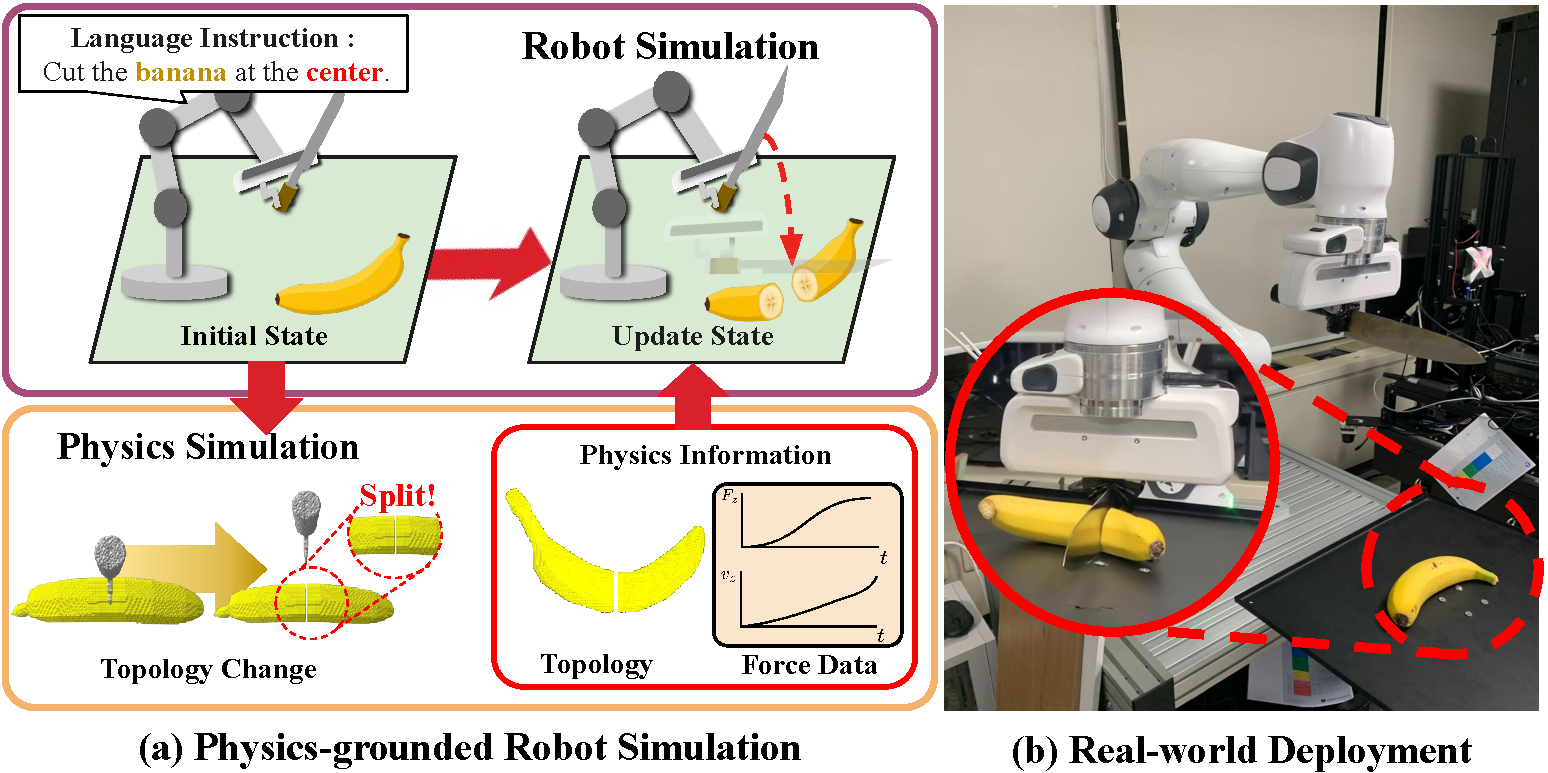
\includegraphics[width=0.95\linewidth]{figure/intro_figure.pdf}
  \caption[{Overview of physics-grounded robotic food cutting}]{\textbf{Overview of physics-grounded robotic food cutting.} IntSim combines robot execution with material deformation and topology changes to generate CulinaryCut demonstrations. The pipeline supports evaluation of contact-rich cutting in simulation and transfer to a real robot.}
  \label{fig:cut_introduction}
\end{figure}

\begin{figure}[!htbp]
  \centering
  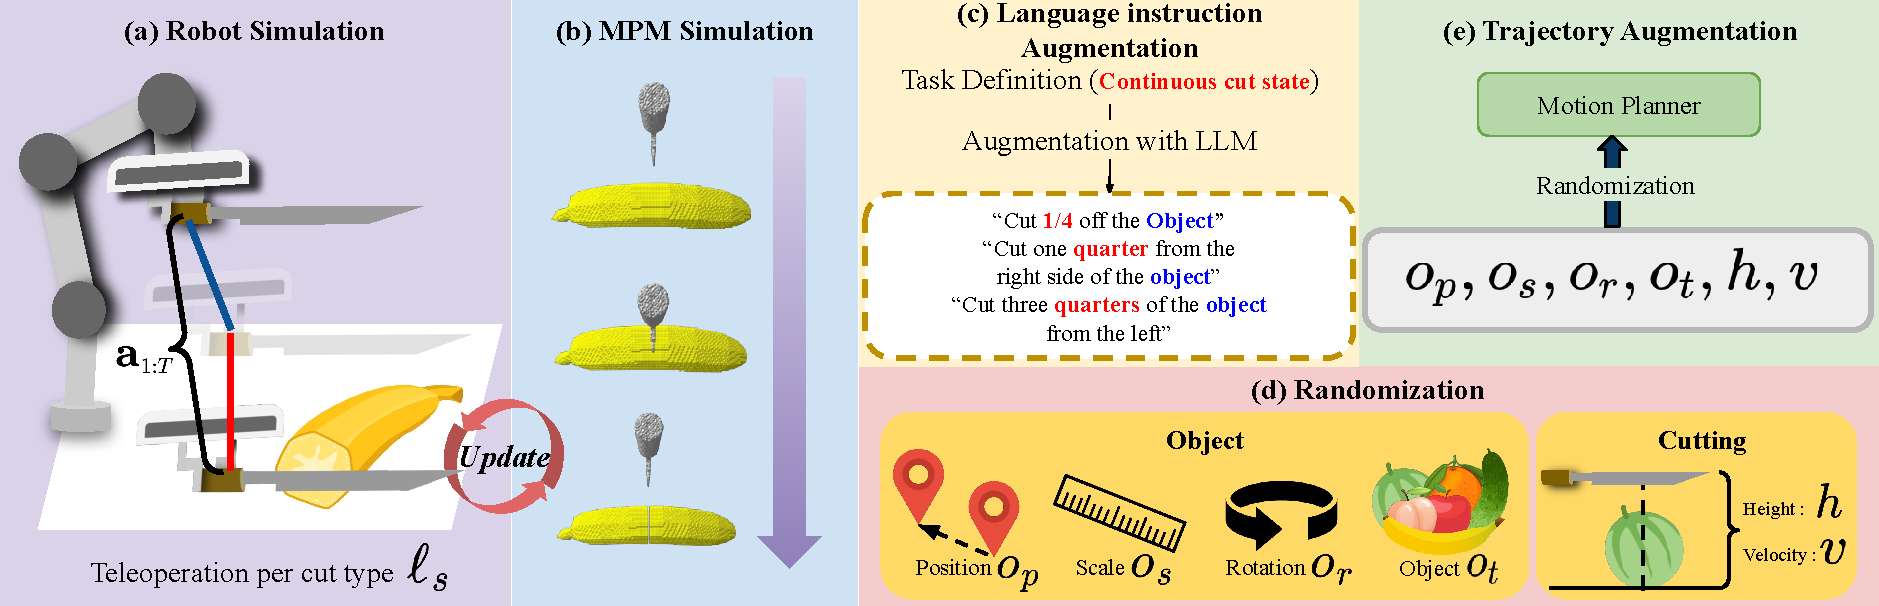
\includegraphics[width=0.96\linewidth]{figure/Method_figure.pdf}
  \caption[{CulinaryCut data generation}]{\textbf{CulinaryCut data generation.} Initial demonstrations and task specifications are converted to cutting motions; IntSim couples ManiSkill robot execution with MLS-MPM material response; language and trajectory augmentation provide diverse geometric configurations and cutting instructions. The benchmark preserves physical contact and topology information while retaining standard VLA action interfaces.}
  \label{fig:cut_pipeline}
\end{figure}

\FloatBarrier

\section{Background and Related Work}
\label{sec:cut_background}

\subsection{Vision--Language--Action Policies and Geometric Supervision}
\label{subsec:cut_related_vla}

VLA models combine visual perception, language understanding, and motion generation in a single learned policy. Representative systems include RT-2~\citep{rt2}, OpenVLA~\citep{openvla}, RDT~\citep{liu2025rdt1bdiffusionfoundationmodel}, Octo~\citep{mees2024octo}, and later generalist-policy architectures such as $\pi_0$~\citep{black2024pi0visionlanguageactionflowmodel}. Their shared objective is to connect a natural-language task description to executable robot actions from visual and, when available, robot-state observations. Although the underlying policy architectures and action encodings vary substantially, most large-scale demonstrations are more naturally suited to measuring object placement, grasping, or reachability than the onset of material separation.

Prior work also explores force-conditioned policy inputs, including ForceVLA~\citep{yu2025forcevla}. CulinaryCut addresses a complementary problem. Rather than asking how much a new force sensor or force-conditioned architecture improves execution, it asks whether existing models acquire more physically effective behavior when the \emph{demonstrations themselves} have been constructed and selected under deformable-material dynamics. The distinction matters when interpreting the results: improved cutting outcomes do not establish that a VLA has learned explicit online force regulation.

\subsection{Manipulation Datasets and Cutting Simulators}
\label{subsec:cut_related_datasets}

General robot datasets such as DROID~\citep{khazatsky2025droidlargescaleinthewildrobot}, Open X-Embodiment~\citep{o2024open}, BridgeData V2~\citep{bridgedata2023}, and LIBERO~\citep{libero2023} provide broad task and scene coverage (Open X-Embodiment also spans 22 embodiments). They are important for training visuomotor representations and language-conditioned behaviors. However, they do not jointly emphasize deformable-material fracture, continuous robot actions, and physical force records in food cutting. Collecting large numbers of real cutting demonstrations is also constrained by safety, tool wear, material variability, and the practical need to repeatedly prepare and replace food objects.

Several simulators and benchmarks have directly addressed cutting and deformable manipulation. DiSECt~\citep{disect2022} and SliceIt!~\citep{sliceit2024} employ finite-element approaches to cutting, while TopoCut~\citep{topocut2025} explores MPM-based topology changes. RoboCook~\citep{shi2023robocook} learns tool--dough interaction with graph-network dynamics trained on real point clouds. Each provides a useful contribution to modeling deformation or robotic interaction, but the comparison motivating CulinaryCut is the lack of a single VLA-oriented benchmark combining robot simulation, continuous actions, language instructions, multi-view images, and contact-aware material evolution. Table~\ref{tab:cut_prior_work} compares the principal capabilities of these datasets and simulators.

\begin{table}[!htbp]
  \centering

  \caption[{Capabilities emphasized by representative cutting and manipulation datasets}]{\textbf{Capabilities emphasized by representative cutting and manipulation datasets.} The comparison concerns benchmark capabilities rather than the numerical accuracy of each simulator. ``--'' denotes that the corresponding capability was not identified as part of the referenced benchmark.}
  \label{tab:cut_prior_work}
    \begingroup
  \CutTableSetup
  \begin{tabularx}{\linewidth}{@{}>{\raggedright\arraybackslash}p{0.235\linewidth}*{7}{>{\centering\arraybackslash}X}@{}}
    \toprule
    Dataset or system & \makecell{Physics\\sim.} & \makecell{Robot\\sim.} & \makecell{Data\\origin} & \makecell{Multi-\\cam.} & Language & \makecell{Cont.\\action} & Cutting \\
    \midrule
    DROID~\citep{khazatsky2025droidlargescaleinthewildrobot} & -- & -- & Real & Yes & Yes & Yes & -- \\
    ARNOLD~\citep{gong2023arnold} & -- & Isaac Sim & Synthetic & Yes & Yes & Yes & -- \\
    RoboChop~\citep{dikshit2023robochop} & -- & -- & Real & -- & -- & -- & Yes \\
    RoboCook~\citep{shi2023robocook} & -- & -- & Hybrid & Yes & -- & -- & Yes \\
    \citet{jamdagni2021robotic} & FEM & -- & Hybrid & -- & -- & -- & Yes \\
    SliceIt!~\citep{sliceit2024} & FEM & Gazebo & Synthetic & -- & -- & Yes & Yes \\
    DiSECt~\citep{disect2022} & FEM & -- & Synthetic & -- & -- & -- & Yes \\
    TopoCut~\citep{topocut2025} & MPM & -- & Synthetic & -- & -- & -- & Yes \\
    \textbf{CulinaryCut} & \textbf{MPM} & \textbf{ManiSkill} & \textbf{Synthetic} & \textbf{Yes} & \textbf{Yes} & \textbf{Yes} & \textbf{Yes} \\
    \bottomrule
  \end{tabularx}
  \endgroup
\end{table}

\FloatBarrier

\subsection{Material Simulation and the Visual/Physical Domain Gap}
\label{subsec:cut_related_physics}

The Material Point Method represents a continuum with moving particles whose momentum equations are solved on a temporary background grid~\citep{sulsky1994particle,2013-mpm}. MLS-MPM~\citep{2018-MLSMPM} and APIC~\citep{2015-APIC,jiang2017angular} improve particle--grid transfer, while continuum damage models permit progressive weakening~\citep{2019-cdmpm,10.1145/3340259}. These are established ingredients of IntSim rather than newly proposed numerical methods.

The \emph{visual domain gap} concerns appearance, lighting, and background differences between simulation and reality; domain randomization and world models can mitigate these differences~\citep{tobin2017domainrandomizationtransferringdeep,nvidia2025cosmosworldfoundationmodel}. The separate \emph{physics gap} concerns material resistance, force, and actual separation. Photorealistic images cannot validate the latter, motivating a simulator that explicitly evaluates deformable contact.

\FloatBarrier

\section{IntSim: Physics-Grounded Cutting Simulation}
\label{sec:cut_intsim}

\subsection{Robot--Material Simulation Coupling}
\label{subsec:cut_coupling}

IntSim couples MLS-MPM to a ManiSkill Franka Emika Panda robot. ManiSkill handles poses, commanded motions, and visual observations; MLS-MPM advances food particles under constitutive forces, gravity, and contact with the knife and board. Momentum exchange yields contact-force estimates, while updated geometry exposes whether the motion physically severs the food.

The paired robotic and material representations are shown in Figure~\ref{fig:cut_introduction}, while the complete data-generation process is summarized in Figure~\ref{fig:cut_pipeline}.

The MPM solver uses a Y-up coordinate system, with gravity
\begin{equation}
  \mathbf{g}=(0,-9.81,0)\ \mathrm{m\,s^{-2}}.
\end{equation}
Robot observations and exported end-effector trajectories are transformed to ManiSkill's Z-up convention by exchanging the vertical axes. Unless stated otherwise, task instructions and reported robot trajectories use the Z-up convention.

\subsection{MLS-MPM Formulation}
\label{subsec:cut_mpm}

The material is discretized into Lagrangian particles coupled through an Eulerian background grid. Each particle $p$ stores its position $\mathbf{x}_p$, velocity $\mathbf{v}_p$, mass $m_p$, volume $V_p$, deformation gradient $\mathbf{F}_p$, affine velocity matrix $\mathbf{C}_p$, accumulated plasticity $\alpha_p$, and scalar damage $D_p\in[0,1]$. The affine term improves the fidelity of angular and shear motion during particle--grid transfers~\citep{jiang2017angular}, while the damage field provides a mechanism for softening material near the cutting interface. Particle--grid--particle transfers use a quadratic B-spline kernel over a $3\times3\times3$ node stencil.

\subsubsection{Conservation Laws and Constitutive Response}
At the continuum level, the material obeys the mass and linear momentum balances and the kinematic evolution of its deformation gradient:
\begin{subequations}\label{eq:gov}
\begin{align}
  \dot{\rho}+\rho\,\nabla\!\cdot\!\mathbf{v} &= 0, \label{eq:gov_mass}\\
  \rho\,\dot{\mathbf{v}} &= \nabla\!\cdot\!\boldsymbol{\sigma}+\rho\,\mathbf{g}, \label{eq:gov_mom}\\
  \dot{\mathbf{F}} &= (\nabla\mathbf{v})\,\mathbf{F}. \label{eq:gov_kin}
\end{align}
\end{subequations}
Here $\rho$ is density, $\mathbf{v}$ is material velocity, $\boldsymbol{\sigma}$ is the Cauchy stress, and $\mathbf{g}$ is gravitational acceleration.

We employ fixed corotated elasticity~\citep{stomakhin2012energetically} as the elastic backbone, with optional $J_2$ plasticity treated through a radial-return update. Writing the polar decomposition as $\mathbf{F}=\mathbf{R}\mathbf{S}$, the first Piola--Kirchhoff and Cauchy stresses are given by
\begin{subequations}\label{eq:corot_simple}
\begin{align}
  \mathbf{P} &= 2\mu(\mathbf{F}-\mathbf{R})
    +\lambda(J-1)J\mathbf{F}^{-\mathsf{T}},\\
  \boldsymbol{\sigma} &= J^{-1}\mathbf{P}\mathbf{F}^{\mathsf{T}},
  \qquad J=\det(\mathbf{F}).
\end{align}
\end{subequations}
The Lam\'e parameters are determined by Young's modulus $E$ and Poisson's ratio $\nu$:
\begin{equation}\label{eq:lame}
  \mu=\frac{E}{2(1+\nu)},\qquad
  \lambda=\frac{E\nu}{(1+\nu)(1-2\nu)}.
\end{equation}
The blade-localized damage variable reduces the effective elastic response by scaling the Lam\'e parameters as damage accumulates. This provides progressive material weakening near the knife, while the particle and surface reconstruction steps expose the resulting opening and separation. These choices are a tractable approximation to food cutting rather than a complete microscopic fracture or fiber-tearing model.

\subsubsection{Particle-to-Grid Transfer}
At the beginning of each MLS-MPM time step, the current material configuration is stored on Lagrangian particles. The background grid is then populated by transferring each particle's mass and momentum to its neighboring nodes through quadratic B-spline weights. In three dimensions, each particle influences a $3\times3\times3$ stencil. Reconstructing grid quantities in this fashion allows the solver to evaluate continuum dynamics without maintaining a mesh whose elements deform permanently with the food.

The affine velocity matrix $\mathbf{C}_p$ carries a local first-order description of particle motion. Including it in the particle-to-grid transfer helps preserve rotational and shear behavior that would otherwise be lost through repeated interpolation. Internal forces are generated from the particle deformation state through the fixed corotated constitutive law, and the material response is modified when yielding or local damage is active. In cutting, this stage links the evolving internal state of the food to the forces that influence the subsequent grid velocity update.

\subsubsection{Grid Evolution and Tool Contact}
After the particle-to-grid transfer, grid velocities are formed from the accumulated nodal momentum and mass. External acceleration, including gravity, is applied at the grid level. Boundary handling and mild numerical stabilization further constrain the velocity field before the updated grid state is transferred back to the particles.

The knife and cutting board are represented by signed distance fields (SDFs). For a position in the active region, the sign and magnitude of the SDF determine whether the corresponding location lies inside or outside a tool and its distance from the surface. Contact queries are restricted to each tool's axis-aligned bounding box to avoid evaluating blade or board geometry throughout the entire computational domain. At candidate contact nodes, the relative tool--material velocity is decomposed into normal and tangential components. Non-penetration, restitution, and Coulomb-friction responses are then applied to determine the post-contact motion.

The velocity impulse generated by contact is accumulated and divided by the corresponding measurement interval $\Delta t_{\mathrm{acc}}$ to estimate mean contact force:
\begin{equation}\label{eq:force}
  \mathbf{F}_{\mathrm{avg}}=
  \frac{1}{\Delta t_{\mathrm{acc}}}
  \sum_{i\in\mathcal{C}}m_i
  \bigl(\mathbf{v}_i^{\mathrm{after}}-\mathbf{v}_i^{\mathrm{before}}\bigr),
\end{equation}
where $\mathcal{C}$ denotes the material degrees of freedom contributing to the contact impulse over the accumulation interval. The equal-and-opposite reaction acts on the tool; reported force magnitudes refer to the contact interaction rather than the static robot-arm sensor load. This impulse-based measurement is recorded alongside generated trajectories but is not a VLA observation at inference time.

The implementation uses a normalized contact-strength indicator $\hat c\in[0,1]$ to gate blade-localized damage and to modulate a material-dependent knife-resistance update. The update depends on the approach speed and material properties, so geometrically similar cutting trajectories may produce different responses across materials. The contact normalization and resistance-update equation are provided in Appendix~\ref{app:cutting-impl}, Eq.~\eqref{eq:cut_resistance}.

\subsubsection{Grid-to-Particle Transfer and Deformation Update}
Updated grid velocities are interpolated back to particles to compute particle velocities and affine velocity matrices. A small blade-tip separation term is applied in a narrow edge band to mitigate numerical sticking and promote crack opening. The deformation gradient is then advanced by
\begin{equation}\label{eq:Fupdate}
  \mathbf{F}_p^{n+1}=\bigl(\mathbf{I}+\Delta t\,\mathbf{C}_p^{n+1}\bigr)
  \mathbf{F}_p^n.
\end{equation}
The implementation additionally applies a volume-normalization safeguard to deformation gradients whose Jacobian leaves a specified safe interval, using the rescaling $\mathbf{F}\leftarrow J^{-1/3}\mathbf{F}$. This operation restores unit determinant; it should not be interpreted as a constitutive plasticity update.

\subsection{Damage-Gated Separation and Numerical Stability}
\label{subsec:cut_damage}

Damage is updated only for particles in a narrow blade-SDF band $|\phi|<b$, and only when the following conditions hold simultaneously: (i) contact strength exceeds a threshold $\hat c\ge\hat c_{\min}$, (ii) the material approaches the blade sufficiently quickly, $v_n\le-v_{\mathrm{th}}$, and (iii) the tool is executing a downward cutting stroke. As damage accumulates, local stiffness decreases; particle-connectivity or color-based surface updates stabilize the visual representation of separated regions.

To account for changes in numerical resolution, the blade-SDF band and approach-speed threshold are adjusted using grid-spacing and time-step scales. The solver uses a CFL-limited time step together with speed caps, damping, bounded deformation determinants, and local SDF-query culling. The precise scaling rules and time-step bound are given in Appendix~\ref{app:cutting-impl} (Eqs.~\eqref{eq:cut_resolution_scaling} and~\eqref{eq:cut_cfl}). The GPU implementation uses Taichi~\citep{hu2019taichi} kernels and atomic reductions for contact impulses. In addition to the generated image/action data, diagnostic records include force--time curves, deformation-Jacobian statistics, contact-strength traces, impulse checks, and simulation parameters.

\begin{figure}[!htbp]
  \centering
  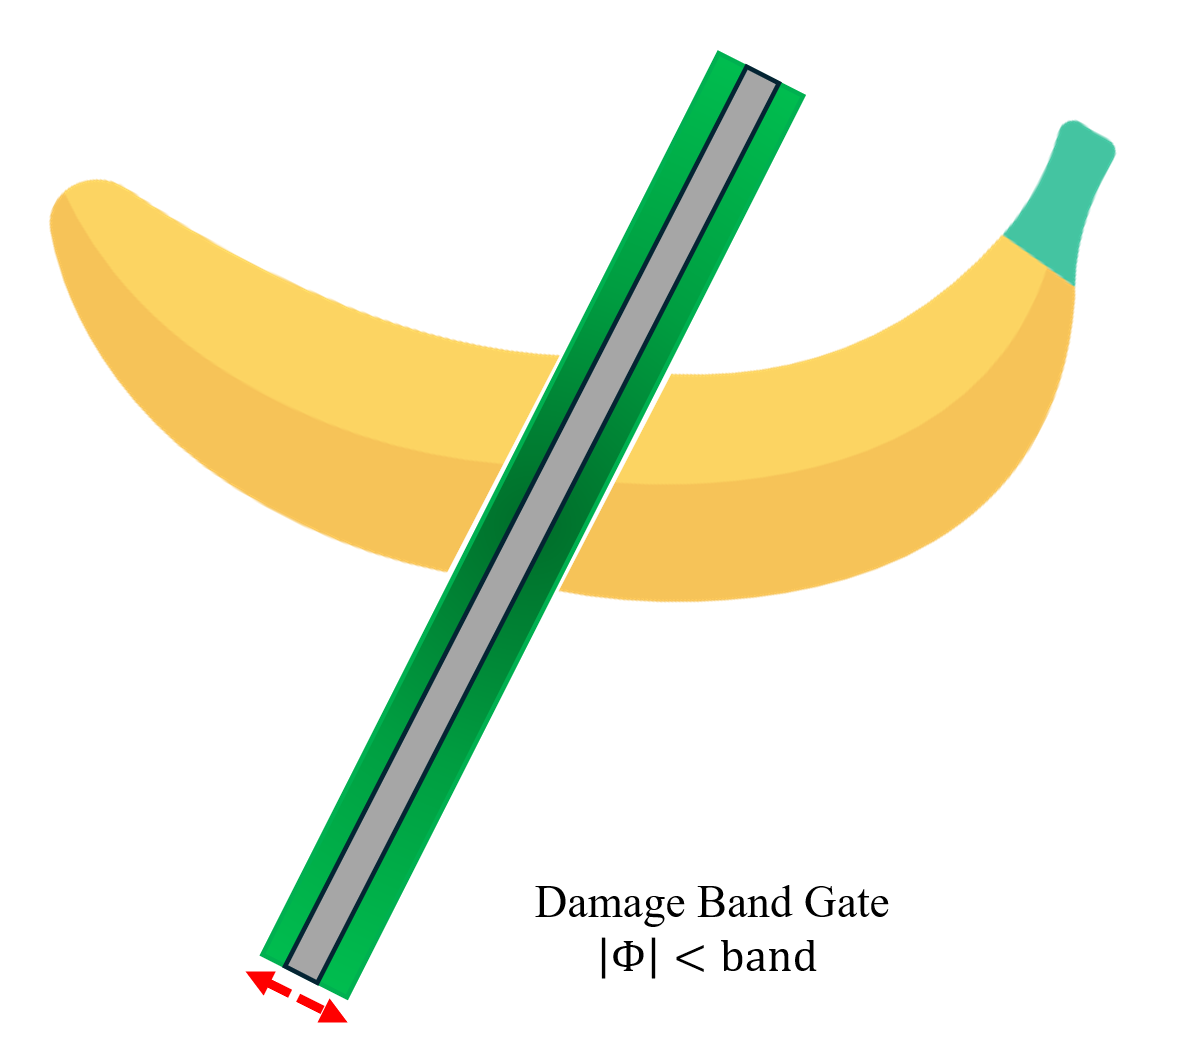
\includegraphics[width=0.65\linewidth]{figure/MPM_Simcut_Figs.png}
  \caption[{Blade-localized damage gate}]{\textbf{Blade-localized damage gate.} Damage is accumulated in a signed-distance band surrounding the cutting tool when contact-strength, approach-speed, and stroke-direction criteria are satisfied.}
  \label{fig:cut_damage_gate}
\end{figure}

\FloatBarrier

\subsection{Implementation Diagnostics and Resolution Treatment}
\label{subsec:cut_diagnostics}

The implementation also records contact-strength traces, blade/board impulses, and relevant metadata such as $\Delta x$, $\Delta t$, material properties, and end-effector states. When the grid resolution or time increment changes, the SDF-band width, speed threshold, and contact normalization scale are adjusted according to the rules stated above. These choices are intended to maintain interpretable cutting behavior across numerical settings, but they should not be confused with a formal proof that all cutting outcomes are fully resolution independent.

\subsection{Material Parameters and Simulation Settings}
\label{subsec:cut_sim_params}

Where published food-engineering measurements report a material parameter, the simulation takes it from them \citep{kheiralipour2008some,mattos2005heat,nourain2005firmness,jahanbakhshi2020determination,kurniawati2023determination,kabas2015determination,an2025relationship}; the remaining parameters are set for the simulation, and Table~\ref{tab:cut_material_properties} marks which values come from each source. The material solver operates over a $0.5\times0.5\times0.5$\,m domain, spanning $[-0.25,0.25]\times[0,0.5]\times[-0.25,0.25]$\,m in its Y-up frame. A $120^3$ Cartesian grid yields $\Delta x\approx4.17\times10^{-3}$\,m, and food particles are initialized at approximately $2.5\times10^{-3}$\,m spacing. The reported base integration time step is $\Delta t=2\times10^{-5}$\,s and is reduced automatically when required by the stability criterion. The robot simulation provides the Franka arm, its knife, table, and visual observations.

The robot environment renders multi-view RGB observations and records end-effector position and velocity alongside simulated contact-force logs. Its representative camera is located at $\mathrm{eye}=(0.5,0.3,0.5)$\,m, looking toward $(0.0,0.1,0.0)$\,m with a $35^{\circ}$ field of view. The observation stream is reported at 60 fps, with six substeps per output record; the output cadence is decoupled from the CFL-controlled material integration step. For VLA fine-tuning, the particular baseline may use a restricted view and a model-specific control frequency, as described below.

Table~\ref{tab:cut_discretization} summarizes the main simulation and observation parameters. The fact that the food particles are spaced more densely than the MPM grid is not inconsistent: particles encode material samples and histories, while the computational grid carries temporary masses, momentum, and stress forces. Both scales must be specified to interpret the spatial detail visible in the particle galleries and the numerical resolution of the solver.

\begin{table}[!htbp]
  \centering
  \caption[{Representative IntSim numerical and observational settings}]{\textbf{Representative IntSim numerical and observational settings} , used for the representative IntSim configuration. Spatial and temporal quantities refer to different parts of the coupled pipeline.}
  \label{tab:cut_discretization}
  \begingroup
  \CutTableSetup
  \begin{tabularx}{\linewidth}{@{}>{\raggedright\arraybackslash}p{0.43\linewidth}X@{}}
    \toprule
    Quantity & Reported setting \\
    \midrule
    Material grid & $120^3$ nodes \\
    Domain side lengths & $0.5\times0.5\times0.5$\,m \\
    Grid spacing $\Delta x$ & $4.17\times10^{-3}$\,m (approx.) \\
    Particle spacing $\Delta x_p$ & $2.5\times10^{-3}$\,m \\
    Base physics step $\Delta t$ & $2\times10^{-5}$\,s (CFL-adaptive) \\
    Output rate & 60 fps (reported observation stream) \\
    Reported substeps per output & 6 \\
    Representative camera FOV & $35^{\circ}$ \\
    Board--food friction & $\mu=0.5$ \\
    \bottomrule
  \end{tabularx}
  \endgroup
\end{table}

\begin{table}[!htbp]
  \centering
  \caption[{Representative material parameters in CulinaryCut}]{\textbf{Representative material parameters in CulinaryCut.} The benchmark contains 15 food categories; only the seven representative items for which numerical properties are reported in the paper are shown. The values are those used in the simulation. Unmarked values are reported by the source in the last column; $^{\ddagger}$ marks a value chosen within the range that source reports, and $^{\dagger}$ a value set for the simulation because the source reports no value or a different one.}
  \label{tab:cut_material_properties}
    \begingroup
  \CutTableSetup
  \begin{tabularx}{\linewidth}{@{}>{\raggedright\arraybackslash}p{0.2\linewidth}*{3}{>{\centering\arraybackslash}X}>{\raggedright\arraybackslash}p{0.25\linewidth}@{}}
    \toprule
    Food item & Density $\rho$ (kg/m$^3$) & Young's modulus $E$ (MPa) & Poisson's ratio $\nu$ & Source \\
    \midrule
    Apple & $850^{\dagger}$ & $3.0^{\ddagger}$ & $0.33^{\dagger}$ & \citet{kheiralipour2008some} \\
    Cucumber & 980 & $1.0^{\dagger}$ & $0.35^{\dagger}$ & \citet{mattos2005heat} \\
    Melon & $1100^{\ddagger}$ & $1.2^{\ddagger}$ & $0.45^{\dagger}$ & \citet{nourain2005firmness} \\
    Banana & 960 & $0.007^{\dagger}$ & 0.35 & \citet{jahanbakhshi2020determination} \\
    Orange & 1020 & $0.584^{\dagger}$ & $0.24^{\dagger}$ & \citet{kurniawati2023determination} \\
    Peach & 968 & 0.89 & 0.29 & \citet{kabas2015determination} \\
    Strawberry (berry) & 1010 & $0.20^{\ddagger}$ & 0.40 & \citet{an2025relationship} \\
    \bottomrule
  \end{tabularx}
  \endgroup
\end{table}

CulinaryCut uses a single robot arm for cutting, without a second hand to stabilize the food. Passive board--object friction therefore matters: the friction ablation shows that removing board friction (changing $\mu=0.5$ to $\mu=0$) causes approximately $0.034$\,m of center-of-mass drift under an otherwise matched cutting motion. This sensitivity motivates explicit contact and boundary modeling rather than treating the food as a fixed geometric target.

\FloatBarrier

\subsection{Execution-Time Velocity Guardrail}
\label{subsec:cut_guardrail}

To avoid overly aggressive commands during policy evaluation, an external velocity guardrail limits the magnitude of predicted end-effector motion. The guardrail does \emph{not} alter the VLA architecture, supply force feedback to the policy, or replan the target cutting location. Instead, a lightweight regression $\mathcal{R}$ is fit on simulator-generated data spanning knife speeds and material parameters $\mathbf{m}=(E,\sigma_y)$. The predicted peak interaction force determines an allowable motion speed:
\begin{equation}\label{eq:cut_guardrail}
  \hat F=\mathcal{R}(v,\mathbf{m}),\qquad
  v_{\mathrm{safe}}=\max\bigl\{v\mid
    \mathcal{R}(v,\mathbf{m})\le F_{\max}\bigr\}.
\end{equation}
Commands exceeding $v_{\mathrm{safe}}$ are clipped at execution time. The same filter is applied to all evaluated policies, separating this deployment safeguard from any learned force-aware behavior. Its measured effects are reported in Section~\ref{subsec:cut_ablation_guardrail}.

\FloatBarrier

\section{CulinaryCut Benchmark and Training Protocol}
\label{sec:cut_benchmark}

\subsection{Task Design and Geometric Grounding}
\label{subsec:cut_task_design}

The benchmark combines target-object identity, cutting location, directional reference, and cutting style. A ratio-cut instruction specifies a location relative to the object's perceived extent (e.g., ``cut 0.3 of the length from the right''). A middle-cut instruction selects the center. A split-cut instruction requires dividing an object into multiple approximately equal pieces; after the first cut, the remaining geometry changes, and subsequent cut locations must be estimated from the updated object state.

For a one-dimensional object extent of length $L$ measured between its left and right reference points, a left-referenced ratio $r$ and a right-referenced ratio $r$ correspond conceptually to distances $rL$ and $(1-r)L$ from the left endpoint, respectively. Thus the instructions ``0.25 from the left'' and ``0.75 from the right'' describe the same target location. This geometric identity is straightforward in an explicit planner but is not guaranteed to emerge from a policy trained on images and language. In CulinaryCut, left and right references are defined with respect to the camera viewpoint; the planner converts them into a target within the object's estimated extent.

Four cutting styles provide distinct motion profiles: \emph{normal cutting} uses a predominantly downward stroke; \emph{saw cutting} adds periodic lateral oscillation; \emph{bias cutting} adds a sustained lateral displacement during descent; and \emph{guillotine cutting} uses a comparatively rapid vertical stroke. These styles are represented as task and demonstration variations. They are \emph{not} generated by a separately trained Knife Style Transfer Module.

\paragraph*{Normal Cut}
Normal cutting is characterized by an approximately vertical downward movement. In a middle-cut task, the end effector descends once toward the center of the object. In a split-cut task, the motion contains several descending segments, one for each required boundary. Consequently, the trajectories for cutting into three, four, or five pieces differ primarily in the number and location of the individual descents, while retaining the underlying non-oscillatory cutting style.

\paragraph*{Saw Cut}
Saw cutting overlays periodic lateral motion on the downward stroke. We introduce forward--backward horizontal oscillations and randomly sample their frequency for each demonstration. This style changes the local temporal structure of contact and should not be treated as equivalent to a simple straight-line path. It is included as a data-generation variation, not as the output of a separately learned motion-style adapter.

\paragraph*{Bias Cut}
Bias cutting applies a sustained lateral shift while the knife descends. The resulting end-effector path is oblique rather than vertical, thereby modifying the geometry of the knife--material interaction. As illustrated by the trajectory samples, this style can be distinguished from normal cutting directly from the position trace.

\paragraph*{Guillotine Cut}
Guillotine cutting uses a comparatively rapid vertical stroke. Its position-only trajectory can look nearly identical to that of a normal cut; the distinguishing information is largely the time parameterization and associated contact transient. Accordingly, the trajectory figure omits a separate guillotine position trace and explains that the contact-force history carries information that a position-only plot would hide.

\begin{figure}[!htbp]
  \centering
  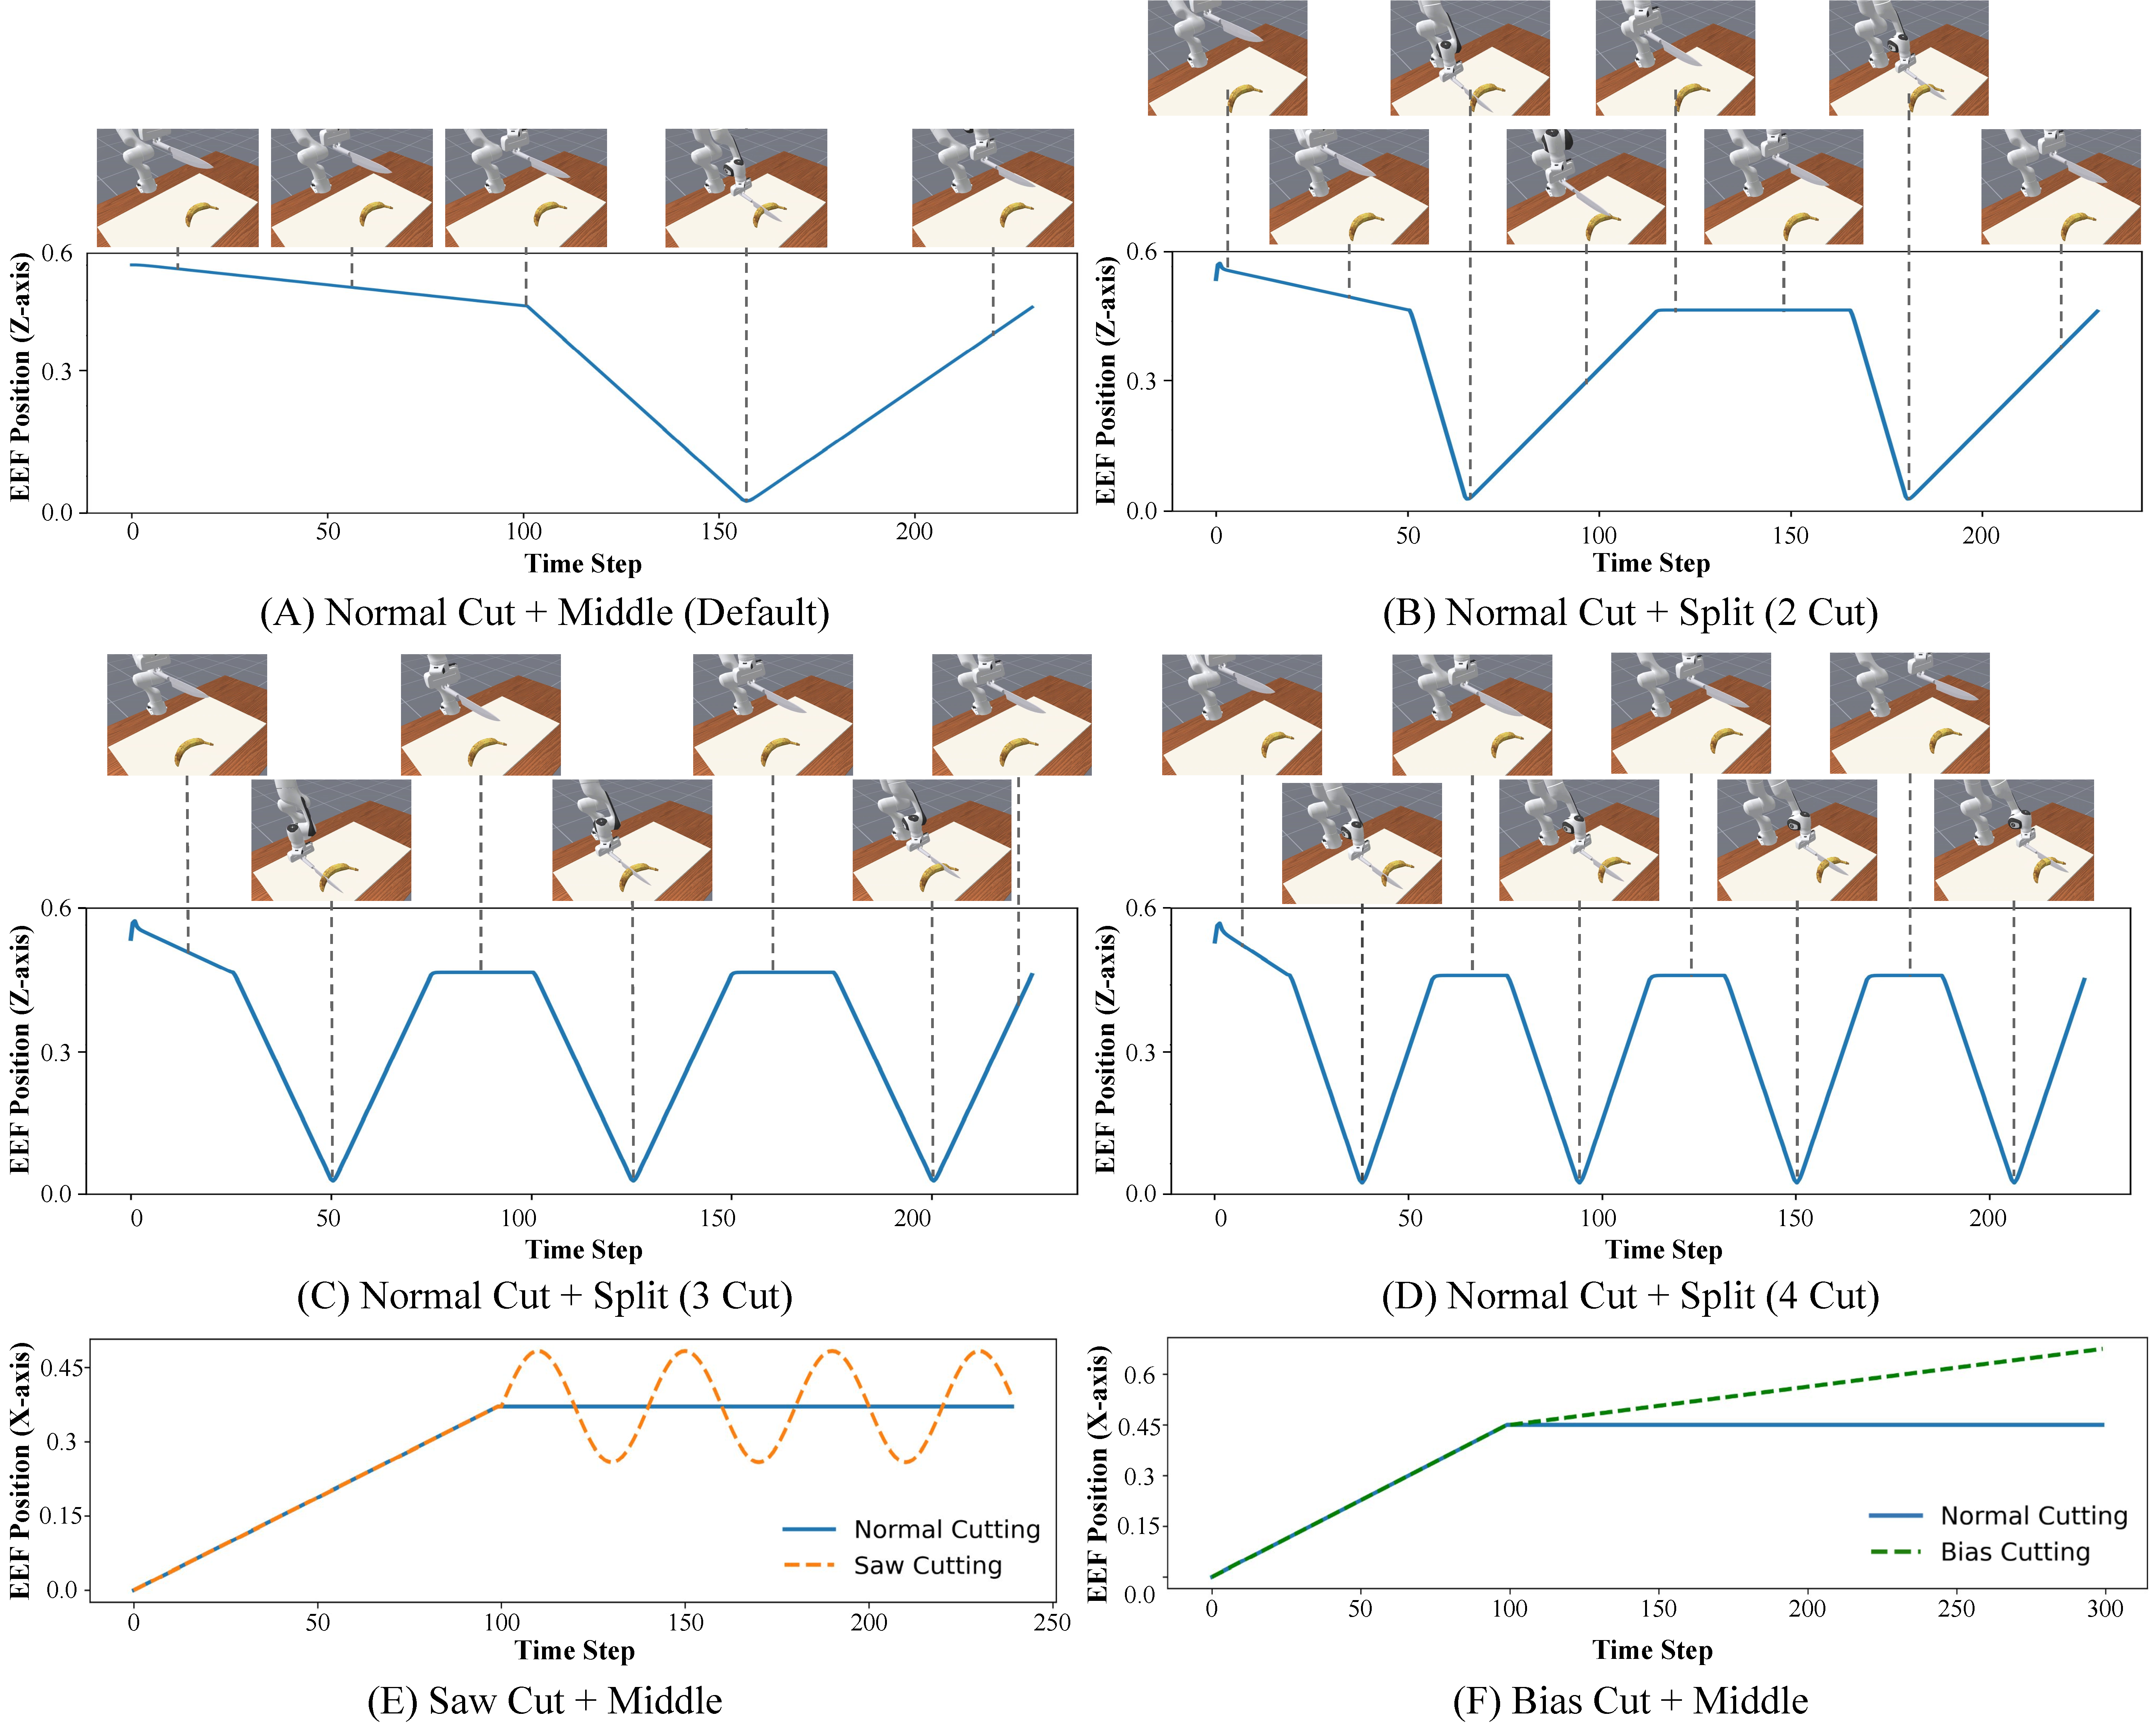
\includegraphics[width=0.95\linewidth]{figure/traj_sample.pdf}
  \caption[{Representative cutting motions}]{\textbf{Representative cutting motions.} Normal cutting follows one or several vertical descents, depending on the cut state; saw cutting adds oscillatory motion, and bias cutting produces a slanted trajectory. Guillotine cutting is primarily distinguished from normal cutting by speed, not its position-only trajectory.}
  \label{fig:cut_trajectories}
\end{figure}

\FloatBarrier

\subsection{Instruction Representation and Ambiguity Resolution}
\label{subsec:cut_language_design}

A cutting instruction is constructed from a \emph{Cutting Specification}: a target food object $O_t$, a motion style $\ell_s$, a cut state, and a directional reference. The cut state may specify a ratio, the middle of an object, or a split into approximately equal pieces. The directional reference describes the perspective from which the target location is measured, such as from the left end, from the right end, or along the principal extent of the object. The full instruction therefore contains more information than the object name and the verb ``cut'': it jointly specifies \emph{what} to cut, \emph{where} to cut it, and \emph{how} the knife should move.

Instructions are assembled using a slot-filling template of the form
\begin{center}
  \texttt{[CUT\_STYLE] [VERB] the [OBJECT] at [POSITION] [DIRECTION]}
\end{center}
where the slots are instantiated using predefined lexical alternatives. Numerical ratios may be expressed with decimals, percentages, or words, and LLM-generated paraphrases provide additional linguistic diversity while preserving the intended cutting specification. Table~\ref{tab:cut_language_examples} gives representative instructions for the twelve style--state combinations. Here $O_t$ denotes the selected target object rather than a literal string shown to a policy.

\begin{table}[!htbp]
  \centering

  \caption[{Representative language instructions in CulinaryCut}]{\textbf{Representative language instructions in CulinaryCut.} The four cut styles are combined with the Ratio, Middle, and Split cut states; the specified reference frame changes the physical interpretation of otherwise similar ratio expressions.}
  \label{tab:cut_language_examples}
    \begingroup
  \CutTableSetup
  \begin{tabularx}{\linewidth}{@{}>{\raggedright\arraybackslash}p{0.17\linewidth}>{\raggedright\arraybackslash}p{0.15\linewidth}X@{}}
    \toprule
    Style & State & Example instruction \\
    \midrule
    Normal & Ratio & Normal cut $O_t$ at a 0.3 ratio from the right. \\
    Normal & Middle & Normal cut $O_t$ at the midpoint along its length. \\
    Normal & Split & Normal cut $O_t$ at the first split boundary from the right. \\
    \midrule
    Bias & Ratio & Bias cut $O_t$ at a 0.4 ratio toward the right end. \\
    Bias & Middle & Bias cut $O_t$ at the midpoint from the left. \\
    Bias & Split & Bias cut $O_t$ at the first split boundary. \\
    \midrule
    Guillotine & Ratio & Guillotine cut $O_t$ at a 0.5 ratio from the left. \\
    Guillotine & Middle & Guillotine cut $O_t$ at the center from above. \\
    Guillotine & Split & Guillotine cut $O_t$ at the first split boundary. \\
    \midrule
    Saw & Ratio & Saw cut $O_t$ at a 0.6 ratio along its length. \\
    Saw & Middle & Saw cut $O_t$ at the midpoint from the right. \\
    Saw & Split & Saw cut $O_t$ at the third boundary toward the right. \\
    \bottomrule
  \end{tabularx}
  \endgroup
\end{table}

The dataset also defines default conventions to keep instructions complete. If only a cut state is specified, the style defaults to \emph{Normal Cut}. If a style is given without a cut state, the state defaults to \emph{Middle Cut}. These defaults are a practical property of the dataset construction process. They prevent an omitted attribute from creating multiple conflicting interpretations during trajectory generation and benchmark evaluation.

\subsection{Trajectory Generation and Dataset Composition}
\label{subsec:cut_dataset}

The generation process begins with cutting demonstrations and task-specific trajectories rather than with a policy that is already capable of successful contact-rich cutting. The generation pipeline combines initial teleoperation examples for each cutting style, an AABB-based motion planner, and material simulation. The planner estimates the target object's spatial extent and maps the language-specified cut state and direction onto an executable cutting position. Object placement and cutting parameters are subsequently varied so that the same command family is not tied to a single initial pose or scene.

Data generation consists of five stages:
\begin{enumerate}
  \item \textbf{Specify the task:} choose object, cut state, style, and directional reference.
  \item \textbf{Plan the knife trajectory:} map the instruction to a target using object geometry and style demonstrations.
  \item \textbf{Simulate contact:} advance ManiSkill and MLS-MPM together, including material resistance and separation.
  \item \textbf{Record the rollout:} store synchronized actions, observations, material states, and force profiles.
  \item \textbf{Augment the data:} vary object states, visual scenes, and language while preserving task semantics.
\end{enumerate}

An important feature of the third stage is that the physical result is not inferred from the requested instruction. A candidate can reach the intended position yet fail to produce material separation. This allows the generation process to distinguish an \emph{intended cut} from an \emph{executed cut}. The comparison between ManiSkill-only and IntSim-grounded training data later uses this distinction as the central experimental variable.

The 15 food items are banana, cucumber, apple, peach, melon, orange, strawberry, pear, kiwi, tomato, lemon, grape, shine muscat, plum, and cherry. The dataset contains 21,000 base trajectories. Each is combined with 15 rendered indoor backgrounds, drawn from ReplicaCAD~\citep{szot2021habitat}, AI2-THOR~\citep{kolve2017ai2}, and ProcTHOR~\citep{deitke2022}, and at least five language realizations. Under the reported expansion protocol, the resulting instance count is
\begin{equation}\label{eq:cut_dataset_size}
  N_{\mathrm{instances}}
   =21{,}000\times15\times5
   =1{,}575{,}000.
\end{equation}
The expanded instances need not represent independent physical rollouts: visual scenes and language variants may reuse the underlying action/material trajectory. Keeping this distinction explicit avoids interpreting augmentation as additional physics simulations.

\FloatBarrier

\subsection{Dataset Preview: Robotic Observations and Particle-Level Cutting}
\label{subsec:cut_dataset_gallery}

The gallery figures serve an important methodological purpose in addition to visual presentation. The upper row for each example is the robot-scene RGB observation generated through ManiSkill; the lower row shows the corresponding MLS-MPM particle configuration. Because the two representations are temporally aligned, they reveal both what a VLA observes and what the material solver computes. The progression of frames makes the distinction between blade motion, local deformation, and visible separation easier to identify than a single final-state image would.

Figure~\ref{fig:cut_gallery_one} contains apple, banana, peach, grape, and cucumber examples. Figure~\ref{fig:cut_gallery_two} adds berry, lemon, orange, and melon. These figures illustrate nine representative foods rather than every one of the fifteen benchmark categories. The purpose is therefore qualitative breadth, not a claim that each material's force response has been calibrated to the same degree. In particular, the images show how the simulator handles different geometry and separation patterns, whereas the real-versus-simulation force experiment is quantitatively reported for banana cutting.

\begin{figure}[!htbp]
  \centering
  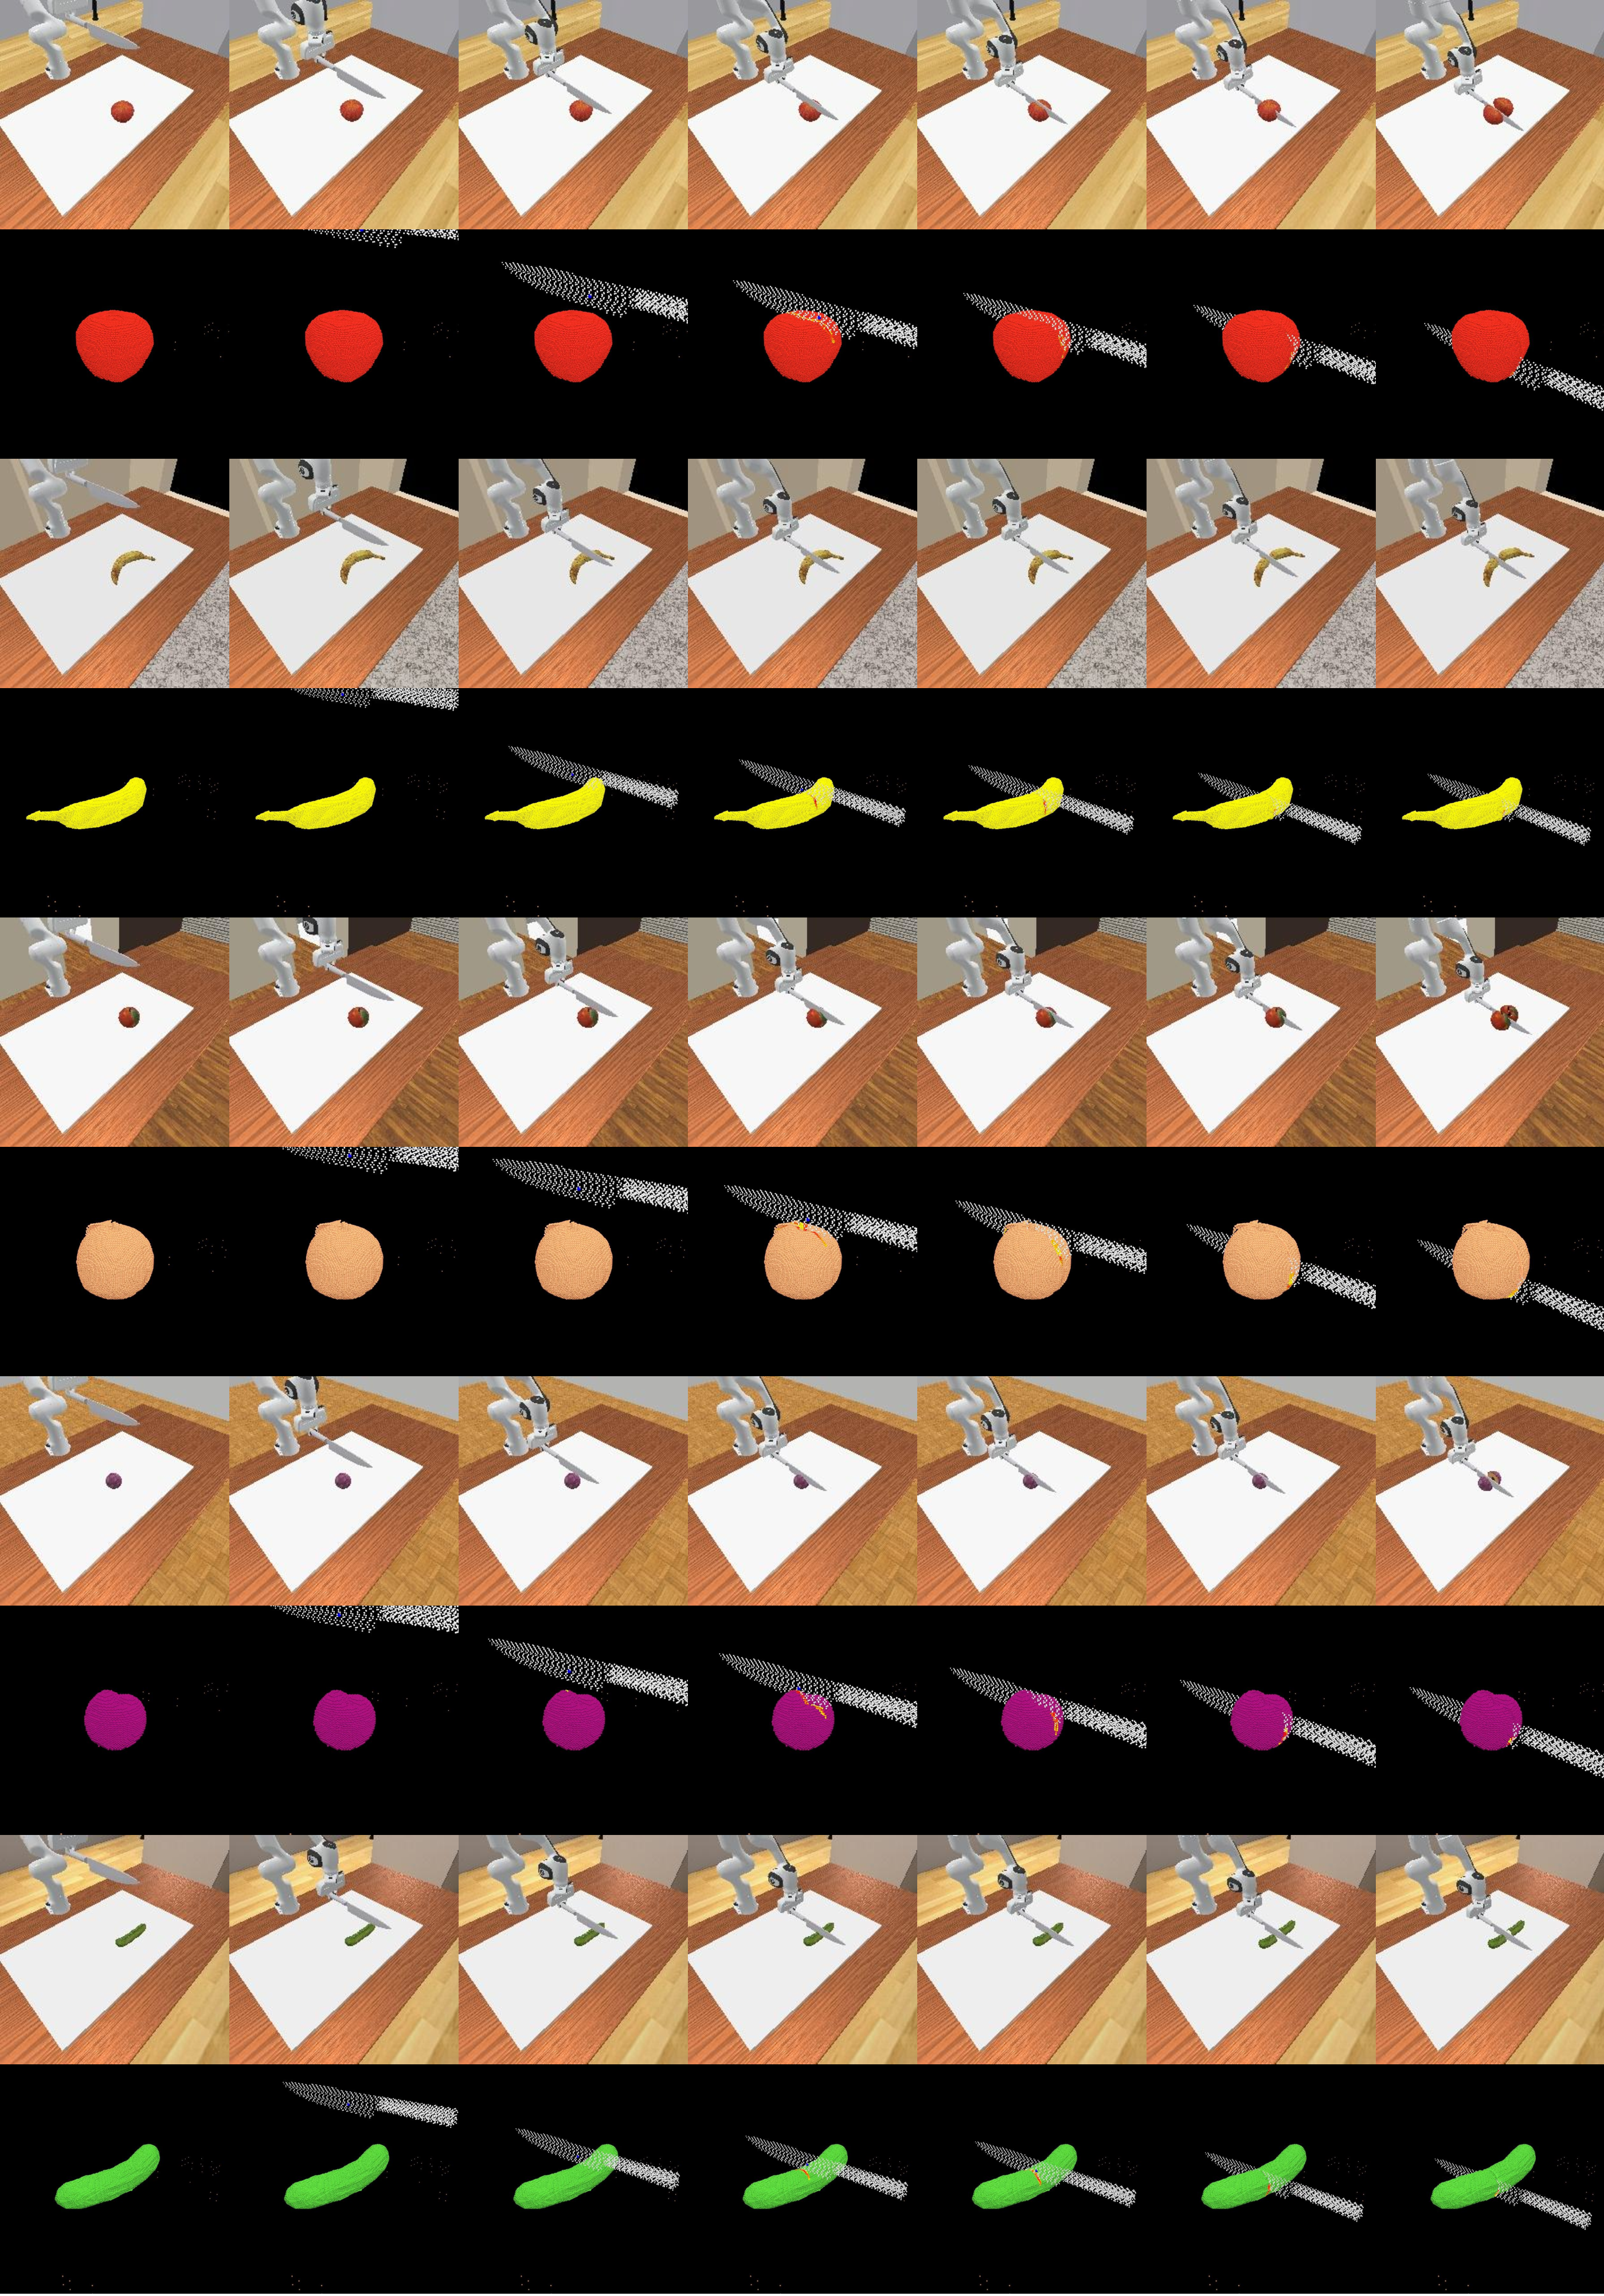
\includegraphics[width=0.84\linewidth]{figure/Gallary.pdf}
  \caption[{CulinaryCut dataset gallery (1/2)}]{\textbf{CulinaryCut dataset gallery (1/2).} Representative cutting sequences for apple, banana, peach, grape, and cucumber. For each food object, the upper row shows temporally ordered RGB observations rendered in ManiSkill with the Franka Panda, blade, and cutting board, while the lower row shows the corresponding MLS-MPM particle configurations. Columns progress from blade approach through deformation to the material-separation stage. The paired views expose particle-level deformation and topology changes that cannot be inferred from robot motion alone.}
  \label{fig:cut_gallery_one}
\end{figure}

\begin{figure}[!htbp]
  \centering
  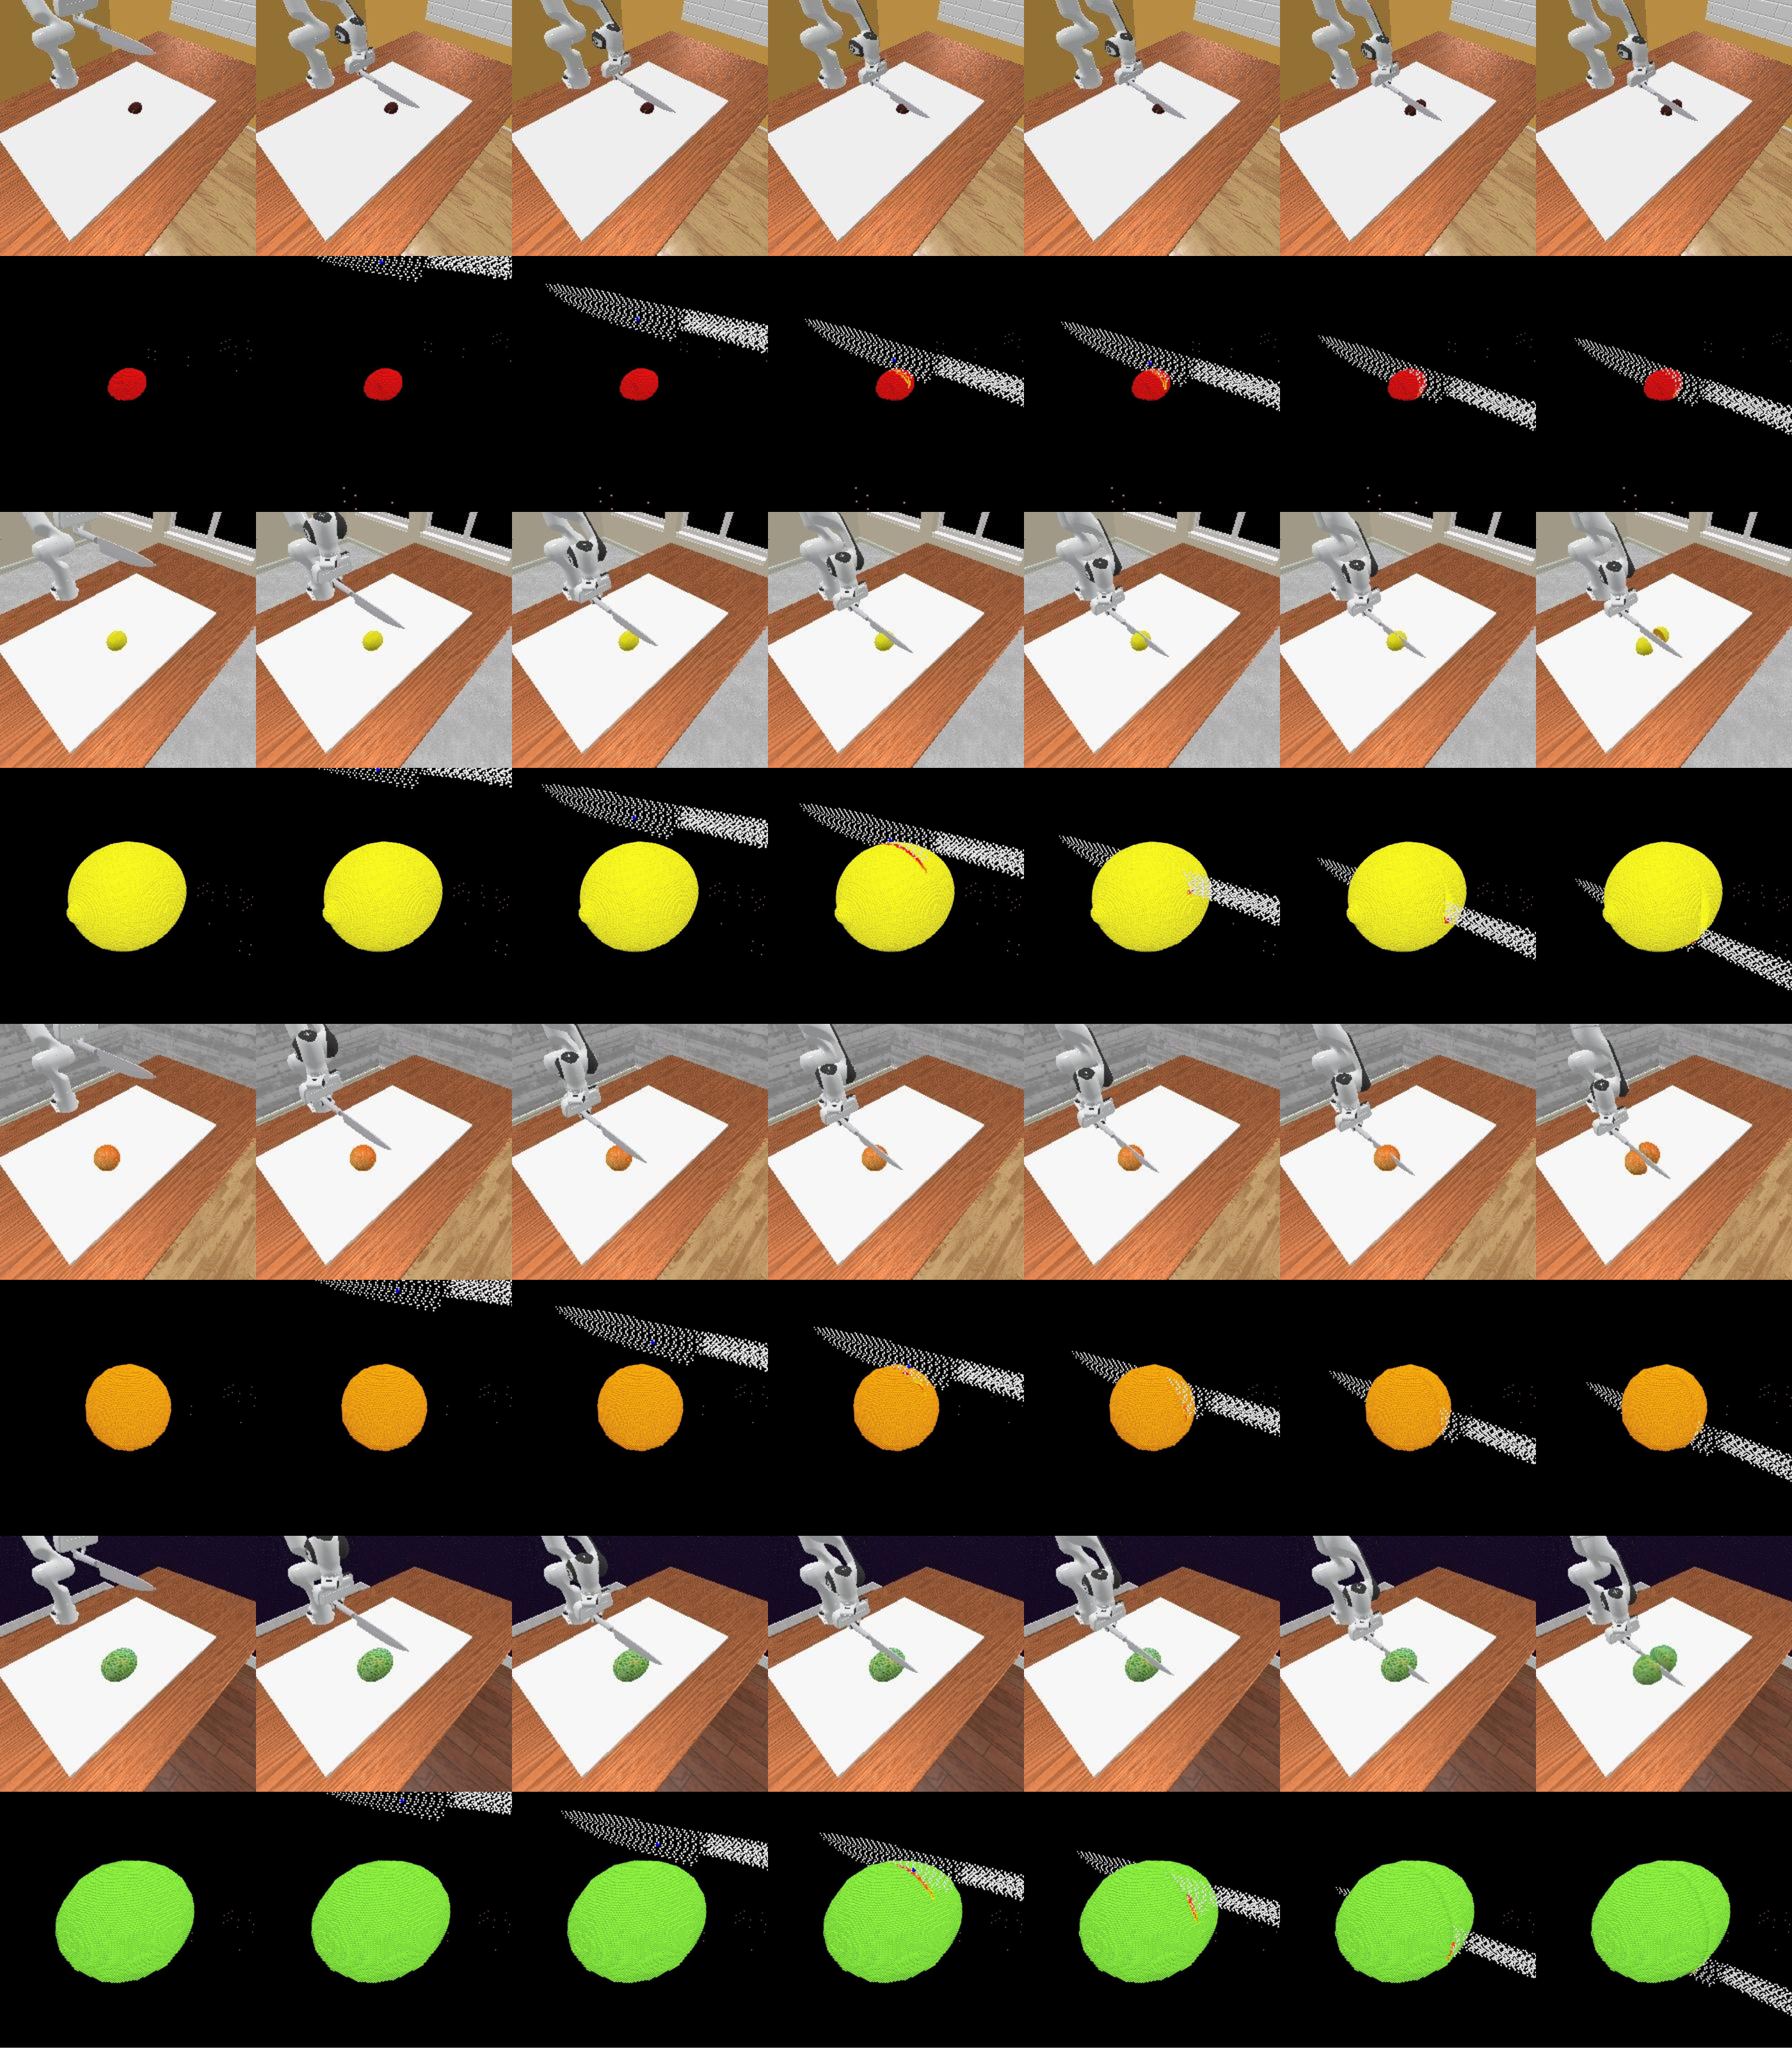
\includegraphics[width=0.88\linewidth]{figure/Gallary_1.pdf}
  \caption[{CulinaryCut dataset gallery (2/2)}]{\textbf{CulinaryCut dataset gallery (2/2).} Additional cutting examples for berry, lemon, orange, and melon, using the same temporally aligned ManiSkill RGB/MLS-MPM particle-view arrangement as Figure~\ref{fig:cut_gallery_one}. The displayed sequences illustrate the material-response pipeline for food objects of different sizes and shapes. These images document simulated deformation and separation; force realism is assessed separately through the real-robot measurements.}
  \label{fig:cut_gallery_two}
\end{figure}

Two observations from the galleries are relevant to the benchmark's design. First, the material's evolving geometry can be a source of supervision or an evaluation criterion even when the VLA itself receives only rendered RGB images. Second, the location that should be cut next may depend on the separation that has already occurred. This becomes particularly important for the topology-update and sequential split-cut experiments, where a policy must interpret the changed scene after its previous action. For a dissertation centered on deformable simulation, these examples also show the scope of the numerical implementation more directly than a table of VLA success rates can.

\FloatBarrier

\subsection{VLA Baselines and Optimization Interface}
\label{subsec:cut_vla}

We fine-tune RDT-1B, Octo, and OpenVLA, abstracting their interfaces as
\begin{equation}\label{eq:cut_policy}
  \hat{\mathbf{a}}_{t:t+H_\pi-1}=\pi_\theta(o_{\le t},\ell),
\end{equation}
where $\ell$ is the instruction and $H_\pi$ the model-specific action horizon. The observation contains supported vision/proprioception, \emph{not} the simulator's force, contact, or damage states. Baseline architectures and fine-tuning settings are retained.

\begin{table}[!htbp]
  \centering
  \caption[{Fine-tuning settings for the three VLA baselines}]{\textbf{Fine-tuning settings for the three VLA baselines.} All three baselines use the front camera as the policy image input.}
  \label{tab:cut_finetune}
    \begingroup
  \CutTableSetup
  \begin{tabularx}{\linewidth}{@{}>{\raggedright\arraybackslash}p{0.34\linewidth}*{3}{>{\centering\arraybackslash}X}@{}}
    \toprule
    Setting & RDT & OpenVLA & Octo \\
    \midrule
    Training scheme & Full fine-tuning & LoRA ($r=32$) & Full fine-tuning \\
    Batch size & 32 & 16 & 128 \\
    Learning rate & $1\times10^{-4}$ & $5\times10^{-4}$ & $3\times10^{-5}$ \\
    Action representation & Joint position & Delta end-effector & Joint position \\
    Action chunk & 64 steps & 1 step & 4 steps \\
    Control frequency & 20 Hz & 5 Hz & 5 Hz \\
    Training updates & 200K & 200K & 1M \\
    \bottomrule
  \end{tabularx}
  \endgroup
\end{table}

\begin{figure}[!htbp]
  \centering
  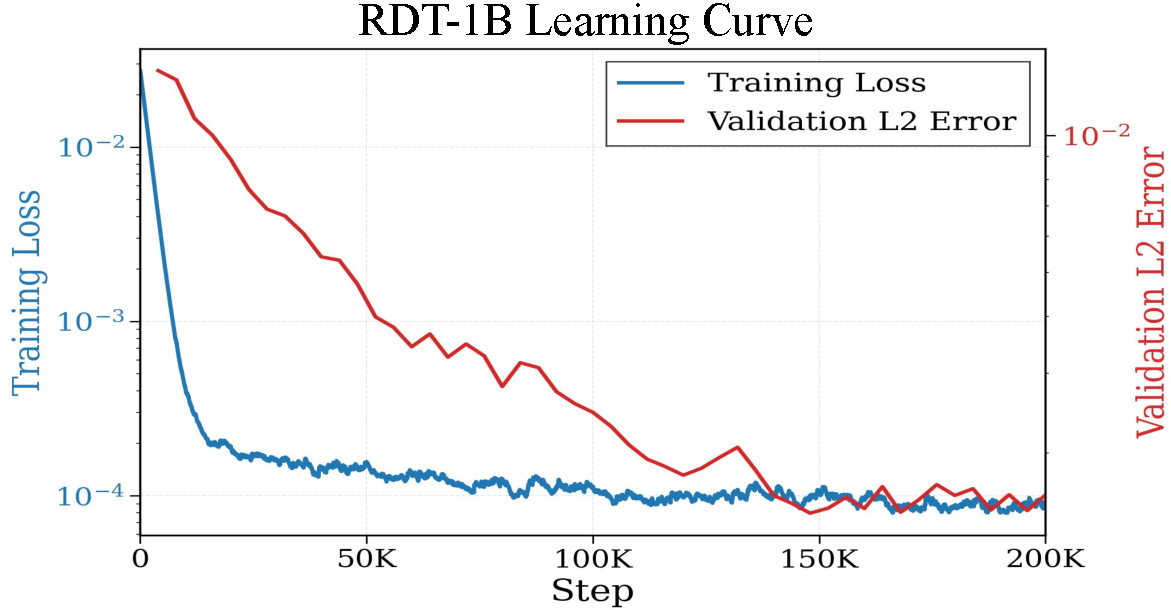
\includegraphics[width=0.75\linewidth]{figure/learning_curve.pdf}
  \caption[{RDT fine-tuning learning curve}]{\textbf{RDT fine-tuning learning curve.} The learning curve provides a qualitative check of RDT fine-tuning convergence.}
  \label{fig:cut_learning_curve}
\end{figure}

To isolate the value of physics-grounded demonstrations, we also compare \emph{the same RDT architecture} trained using two different data sources. The kinematic baseline uses ManiSkill-generated trajectories that satisfy geometric cutting constraints. The physics-grounded variant uses IntSim-generated rollouts selected under MLS-MPM material dynamics. Neither receives forces as policy inputs. This experiment specifically tests whether material-aware behavior can be learned from \emph{physically consistent action trajectories}, rather than from an additional online force-sensing modality.

\FloatBarrier

\subsection{Evaluation Metrics}
\label{subsec:cut_metrics}

Evaluation uses randomized object positions, orientations, and scales, with 20 held-out randomized trials per object/task configuration in the reported simulation protocol. Under the geometry-based criterion, a cut succeeds when the following conditions are satisfied: (i) the knife tip reaches the table within $0.05$\,m positional error; (ii) the blade intersects the intended region; (iii) the blade--object contact angle is within $90^\circ\pm10^\circ$; and (iv) the cutting location is within 10\% of the object's length from the instructed position. Separate physical-severing evaluation within IntSim additionally checks whether the executed trajectory produces an actual cut under deformable-material dynamics.

For real-robot experiments, success is evaluated using both functional penetration and geometric accuracy: the blade must penetrate at least two-thirds of the object's cross-section, and the resulting piece lengths must satisfy the specified cut-location tolerance. These criteria should not be conflated with geometry-only accuracy reported from ManiSkill; the two environments measure different aspects of the same task.

\FloatBarrier

\section{Experiments and Results}
\label{sec:experiment}

\subsection{Visual and Physical Validation of IntSim}
\label{subsec:cut_validation}

Figure~\ref{fig:cut_intsim_visual} shows a representative orange-cutting sequence. ManiSkill supplies the arm and visual scene, while MLS-MPM advances the material state and exposes progressive separation. This example demonstrates why a visual path-following criterion is insufficient: the material dynamics determine whether a knife trajectory actually severs the food.

\begin{figure}[!htbp]
  \centering
  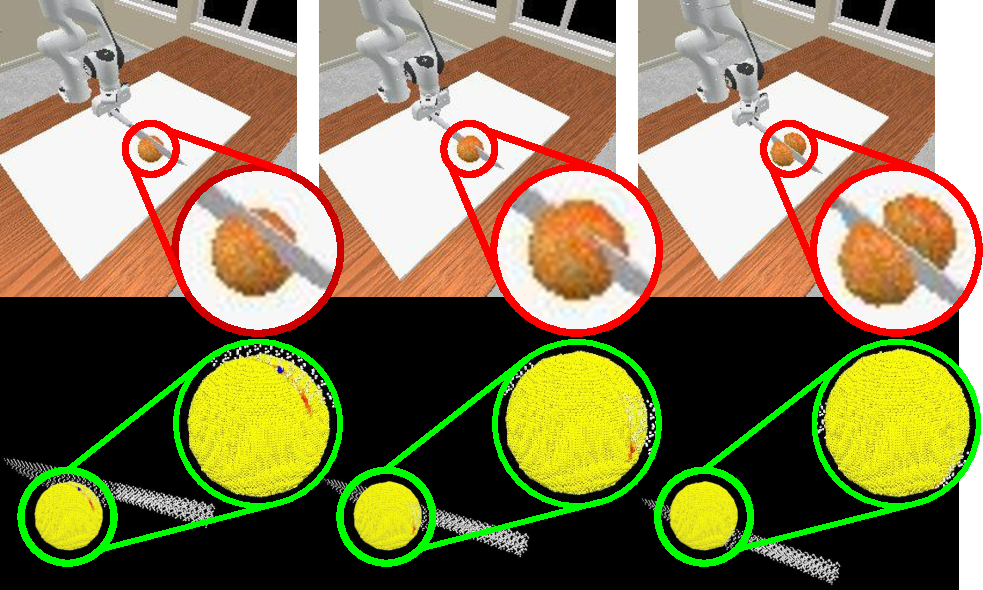
\includegraphics[width=0.88\linewidth]{figure/ms_mpm_eval.pdf}
  \caption[{IntSim material response during orange cutting}]{\textbf{IntSim material response during orange cutting.} The coupled system updates robot motion and particle-level deformation, allowing geometric blade intersection to be distinguished from actual material separation.}
  \label{fig:cut_intsim_visual}
\end{figure}

We also compare simulated knife contact with the vertical reaction force measured during real Franka Panda banana cutting. In a representative experiment, the wrist force/torque sensor exhibits a pre-contact baseline of approximately 25\,N, attributed to tool load and robot-side sensor offset. After baseline subtraction, the real cutting-force peak is approximately 12.5\,N, compared with approximately 12.0\,N from IntSim (less than 5\% relative difference). Normalizing both profiles by their peaks gives similar rise and peak timing, although the release phases differ.

\begin{figure}[!htbp]
  \centering
  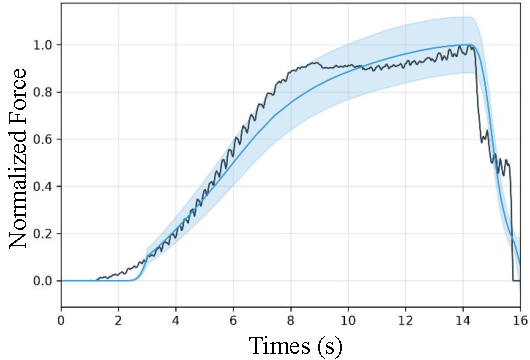
\includegraphics[width=0.78\linewidth]{figure/force_validation_figure_crop.pdf}
  \caption[{Representative force validation against a real Franka robot}]{\textbf{Representative force validation against a real Franka robot.} Real banana-cutting force measurements are compared with IntSim contact-force estimates after accounting for the real sensor's pre-contact baseline. Peak-normalized profiles support temporal comparison.}
  \label{fig:cut_main_force_overlay}
\end{figure}

We also compare force profiles across multiple trials: 20 real banana trials are compared with 30 simulated trials after time rescaling. Their mean profiles share an overall rise--peak--decay pattern, but the simulated mean is smoother and somewhat lower around the cutting transition. This residual discrepancy is consistent with the simplified damage model and numerical smoothing intrinsic to particle--grid transfers; it does not establish fidelity for all materials or cutting styles.

\begin{figure}[!htbp]
  \centering
  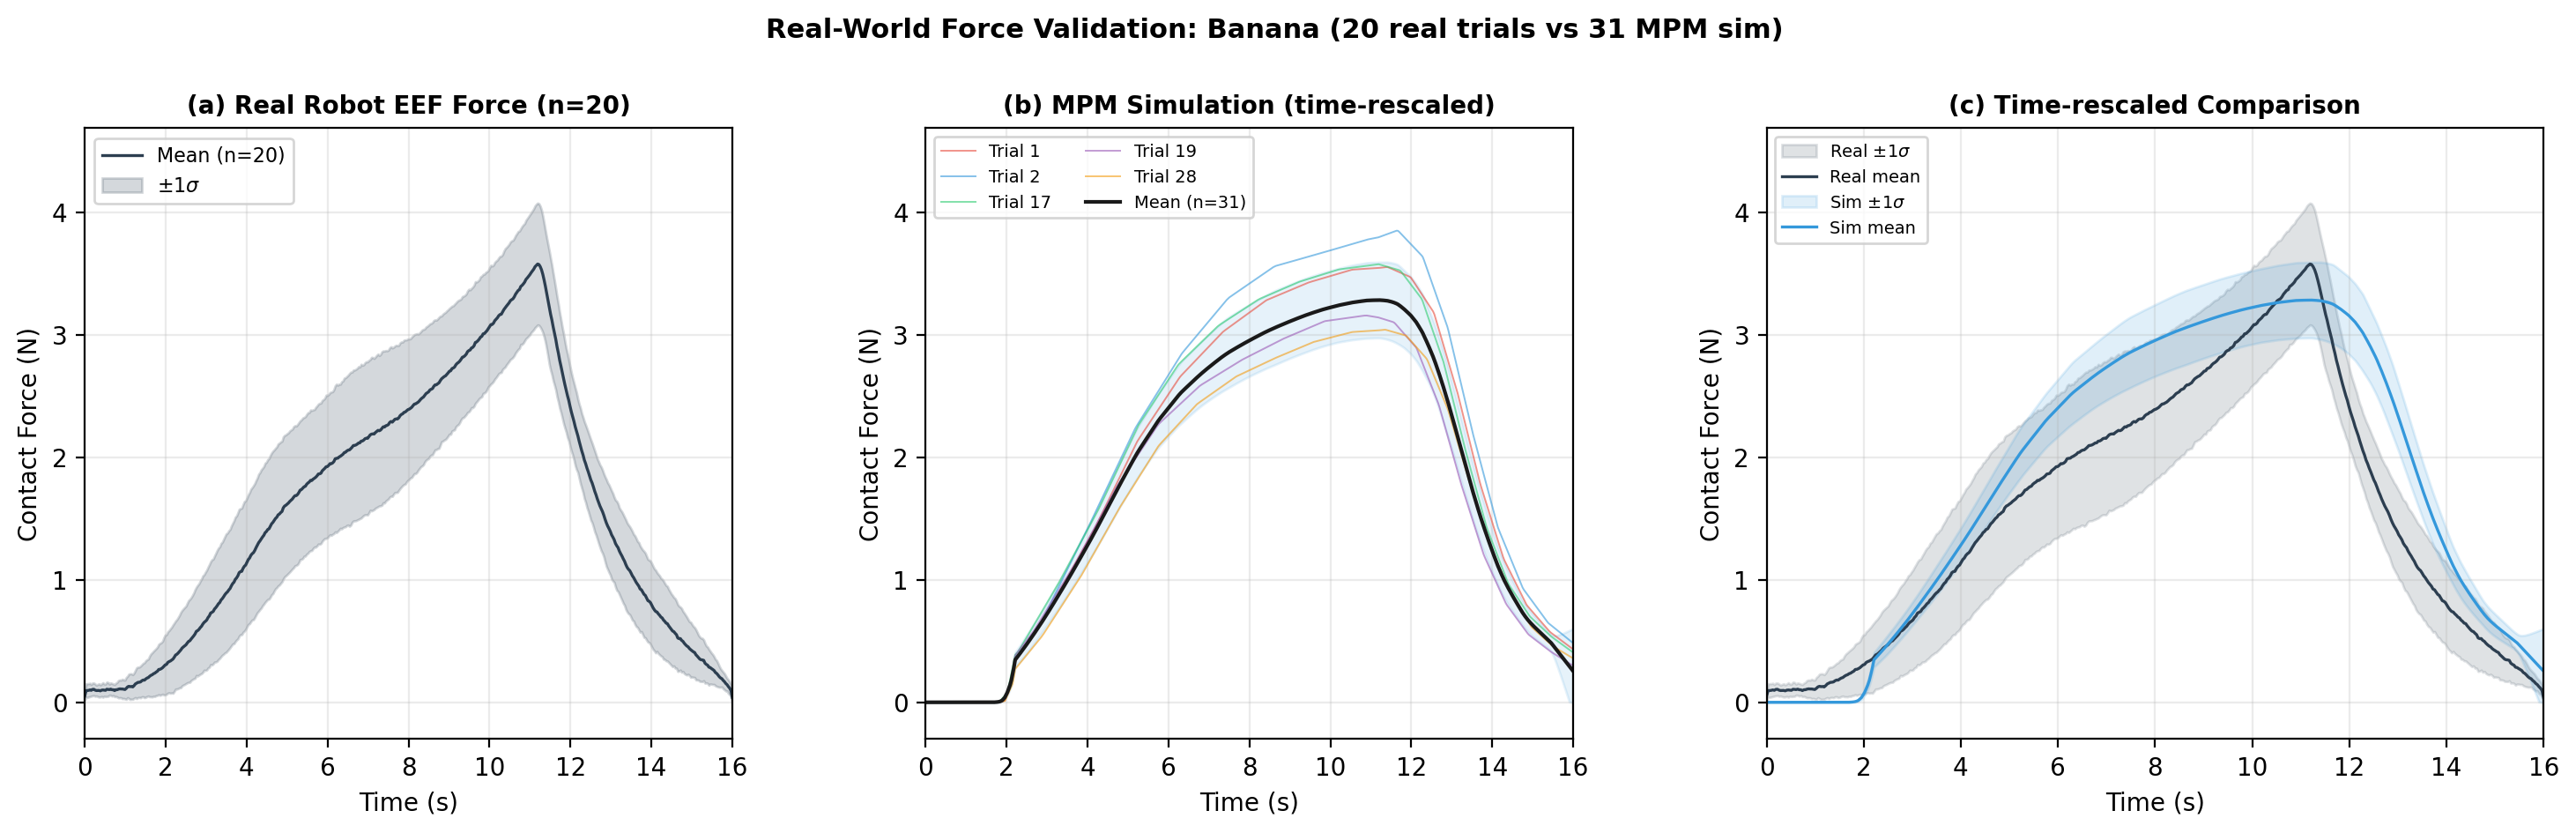
\includegraphics[width=0.91\linewidth]{figure/force_supple.png}
  \caption[{Real--simulation force comparison}]{\textbf{Real--simulation force comparison.} Mean banana-cutting force curves from 20 real and 30 simulated trials, with variation bands, show broadly aligned rise--peak--decay behavior after time rescaling; the simulated cutting transition is smoother. This multi-trial analysis complements the representative peak-force comparison.}
  \label{fig:cut_force_validation}
\end{figure}

\FloatBarrier

\subsection{Geometry-Gap Evaluation}
\label{subsec:cut_geometry_results}

\subsubsection{Object-Scale Sensitivity and Multi-Object Scenes}
Single-object evaluation shows that cutting-point localization varies markedly with object geometry and scale, with smaller objects presenting a particular challenge. Adding distractor foods further degrades target grounding, even when the instruction names the intended target. Table~\ref{tab:cut_geometry_comparison} summarizes geometric generalization performance.

\begin{table}[!htbp]
  \centering
  \caption[{Geometric generalization across evaluation settings}]{\textbf{Geometric generalization across evaluation settings.} Success rates under single-object, multi-object, and held-out-object evaluation conditions.}
  \label{tab:cut_geometry_comparison}
  \begingroup
  \CutTableSetup
  \begin{tabularx}{\linewidth}{@{}>{\raggedright\arraybackslash}p{0.41\linewidth}*{3}{>{\centering\arraybackslash}X}@{}}
    \toprule
    Evaluation setting & RDT & Octo & OpenVLA \\
    \midrule
    Single object & 69\% & 42\% & 51\% \\
    Multi-object scene & 31\% & 17\% & 28\% \\
    Held-out object category & 43\% & 34\% & 26\% \\
    \bottomrule
  \end{tabularx}
  \endgroup
\end{table}

In the multi-object setting, RDT decreases from 69\% to 31\%, Octo from 42\% to 17\%, and OpenVLA from 51\% to 28\%. In leave-one-object-out transfer, performance also drops: RDT reaches 43\%, Octo 34\%, and OpenVLA 26\%. Thus, policies that can execute familiar cutting instructions on known objects remain sensitive to clutter and unseen object appearance or geometry.

\begin{figure}[!htbp]
  \centering
  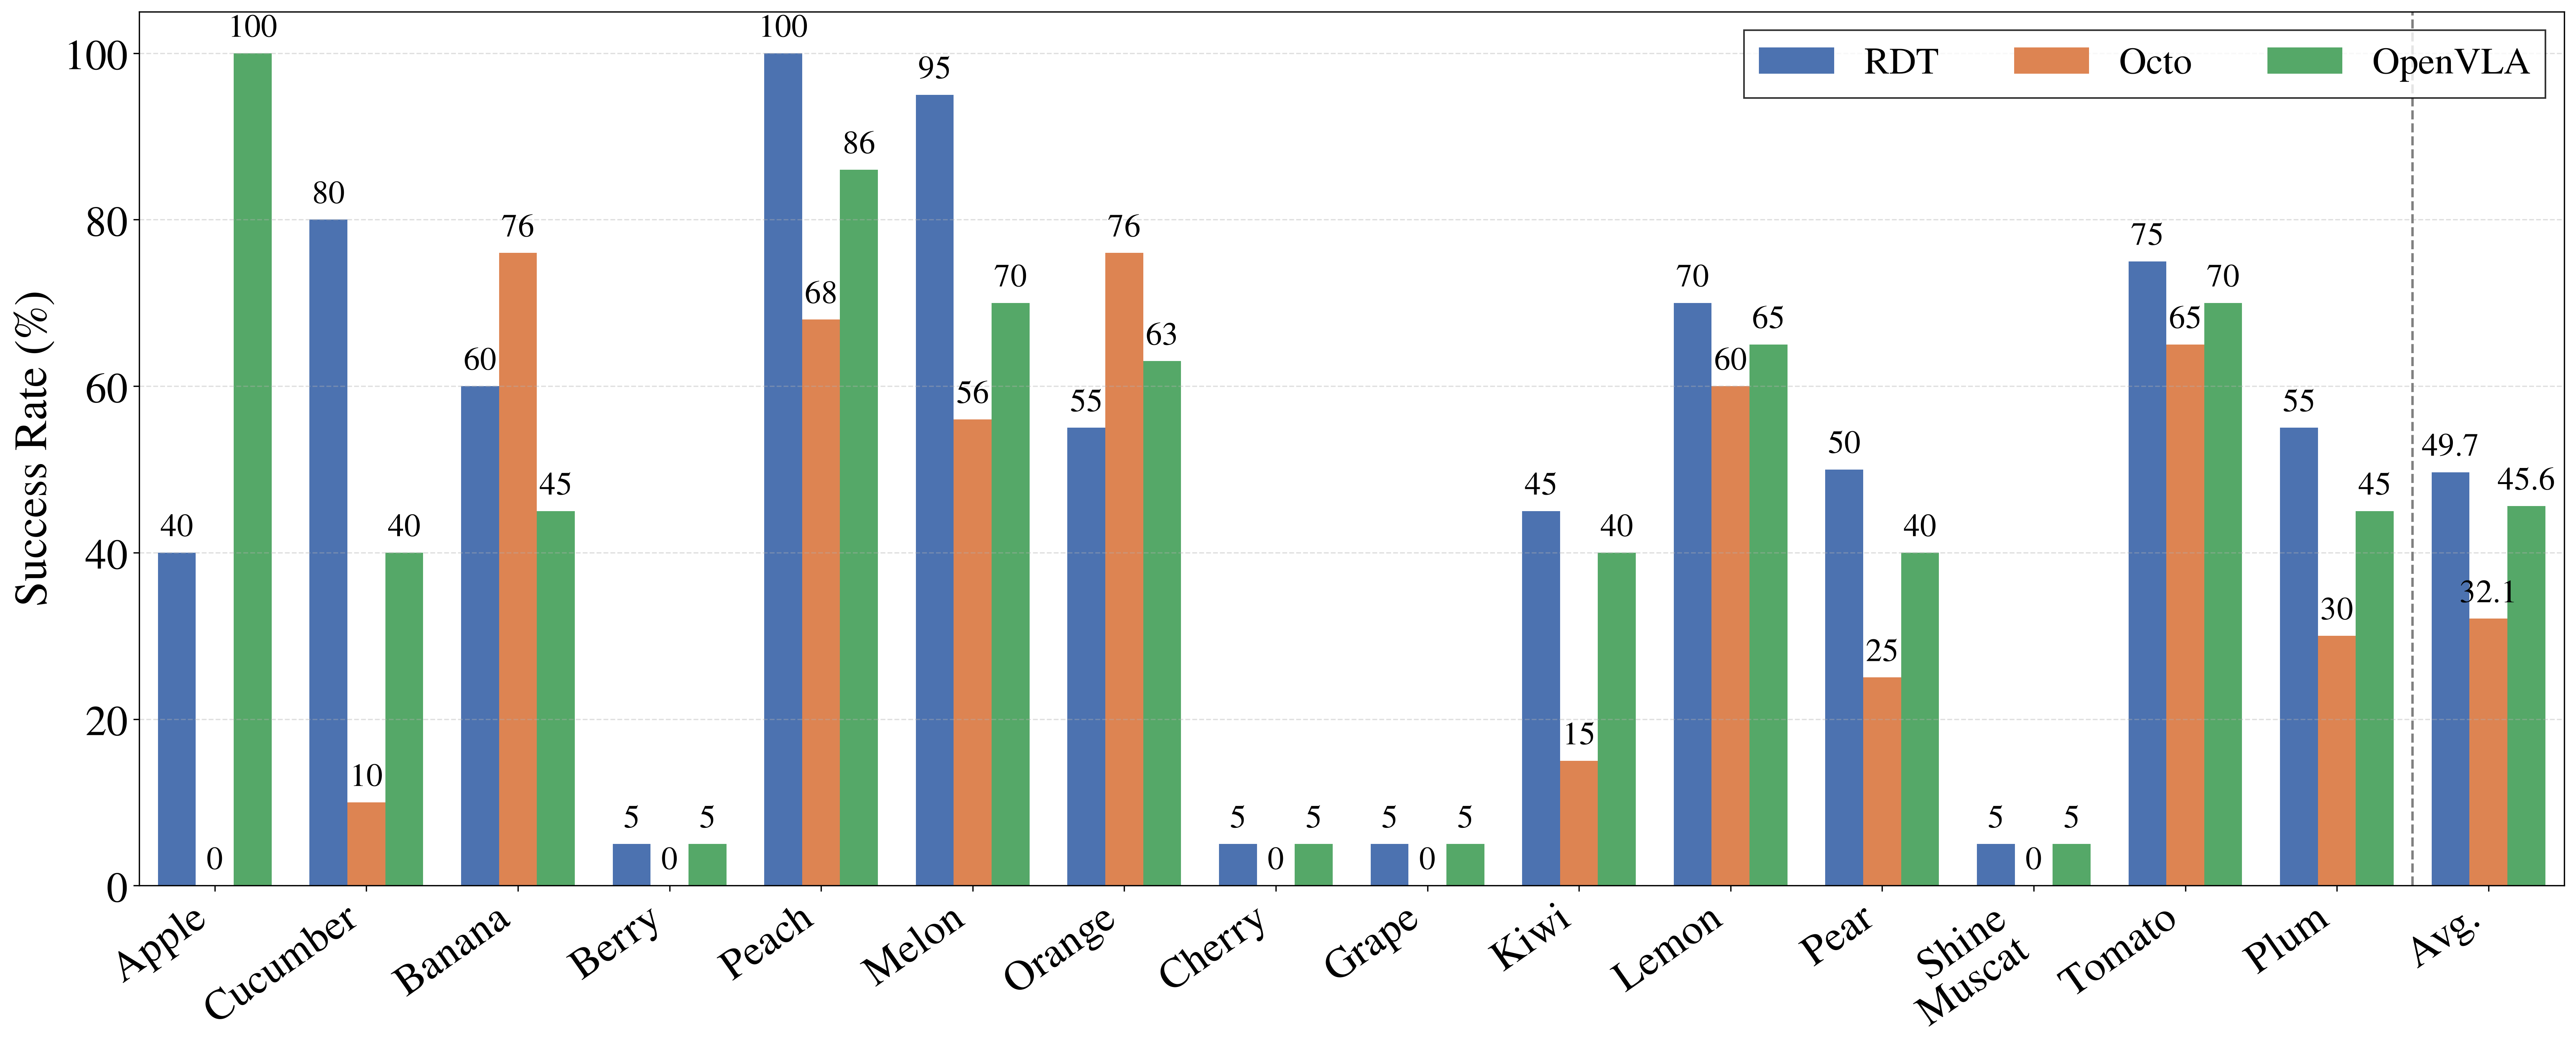
\includegraphics[width=0.92\linewidth]{figure/Add_Object_Variation.png}
  \caption[{Single-object cutting across food categories}]{\textbf{Single-object cutting across food categories.} The experiment compares success rates under variations in food geometry and scale.}
  \label{fig:cut_object_variation}
\end{figure}

\begin{figure}[!htbp]
  \centering
  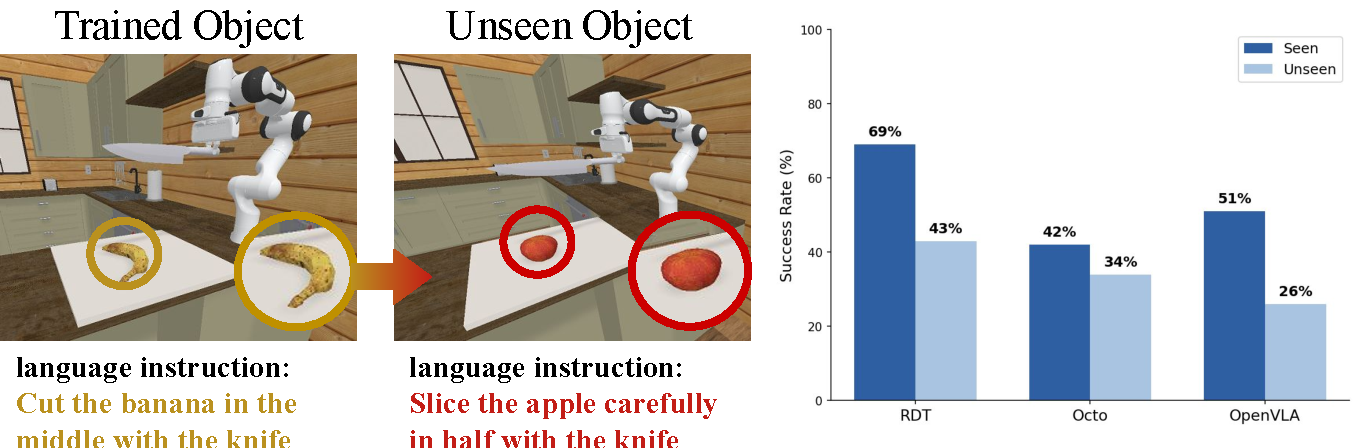
\includegraphics[width=0.84\linewidth]{figure/generalization_transfer.pdf}
  \caption[{Transfer to an unseen food object category}]{\textbf{Transfer to an unseen food object category.} Held-out-category evaluation measures the ability of trained VLA policies to execute cutting motions on objects with previously unseen visual appearance, shape, and material properties.}
  \label{fig:cut_cross_object_transfer}
\end{figure}

\begin{figure}[!htbp]
  \centering
  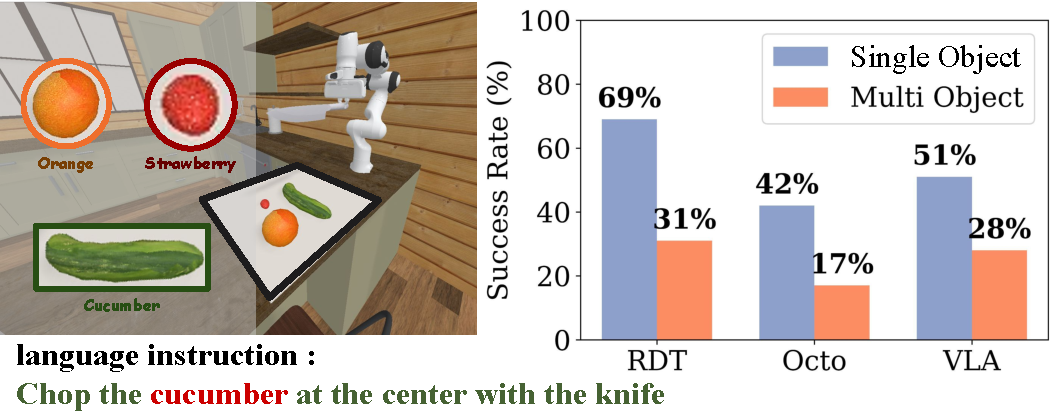
\includegraphics[width=0.85\linewidth]{figure/Multiobjectscene.pdf}
  \caption[{Multi-object geometric grounding}]{\textbf{Multi-object geometric grounding.} The presence of additional food items decreases the probability of selecting and cutting the requested target across all three VLA baselines.}
  \label{fig:cut_multiobject}
\end{figure}

\FloatBarrier

\subsubsection{Continuous Ratios and Directional Reference}
Continuous-ratio evaluation probes whether a policy maps instructions such as ``0.4 from the right'' to an object-centric coordinate. Across ratios between 0.1 and 0.9, performance is unstable even for nearby numerical values, particularly for Octo and OpenVLA. A further RDT transfer experiment shows that accuracy decreases from 55\% to 20\% when the training condition at 0.25 from the right is changed to the tested left-side condition; in the reverse-direction configuration, success decreases from 35\% to 0\%. Transferring from a 0.5-ratio condition to a 0.25-ratio condition reduces success from 60\% to 25\%. These experiments identify shortcomings in jointly representing numerical ratios, directional references, and perceived object extent.

\begin{figure}[!htbp]
  \centering
  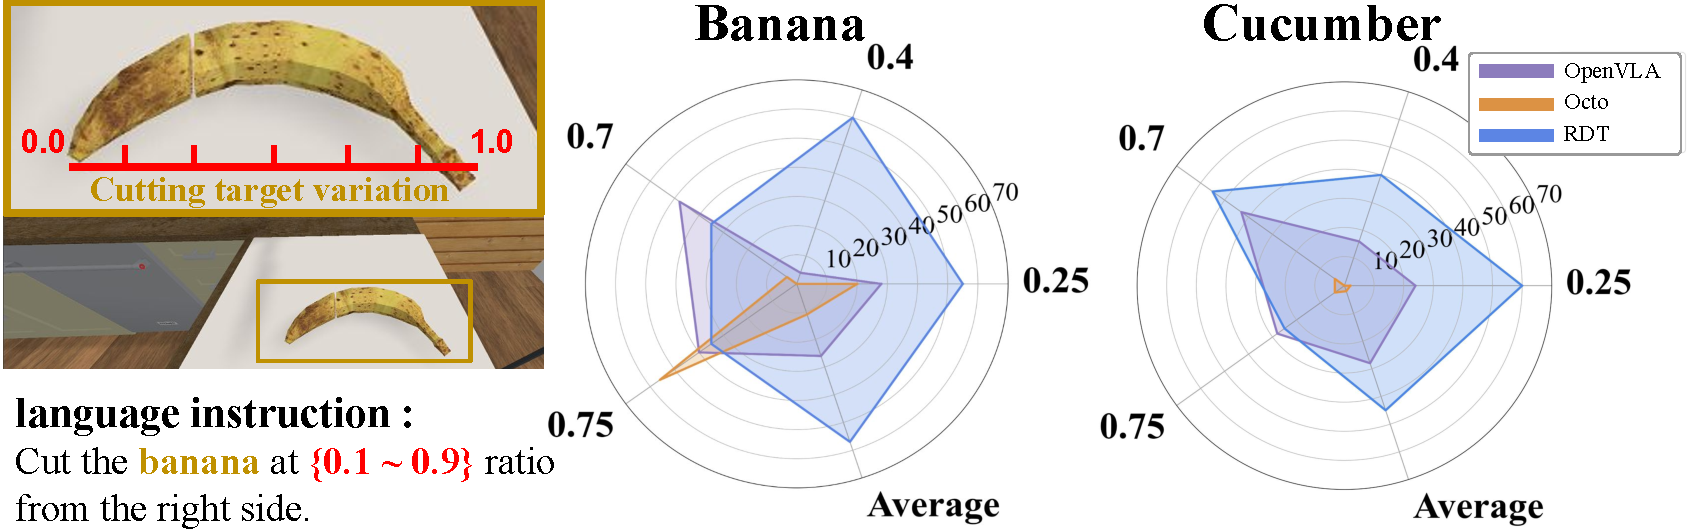
\includegraphics[width=0.94\linewidth]{figure/ContinousCut.pdf}
  \caption[{Continuous-ratio cutting}]{\textbf{Continuous-ratio cutting.} Performance across ratio-conditioned banana and cucumber tasks varies strongly as the requested proportion changes, revealing a geometry-grounding gap despite successful execution at some trained configurations.}
  \label{fig:cut_ratios}
\end{figure}

\begin{figure}[!htbp]
  \centering
  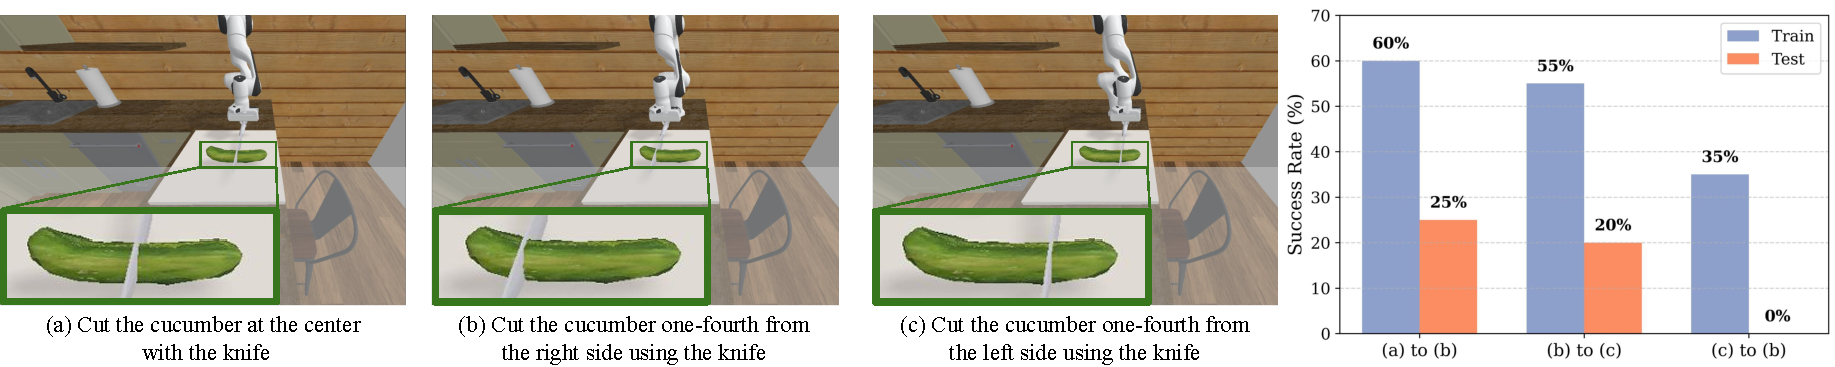
\includegraphics[width=0.90\linewidth]{figure/Transfer Result.pdf}
  \caption[{Directional and ratio transfer}]{\textbf{Directional and ratio transfer.} Transfer experiments compare training and test conditions with different directional references or cut ratios. Accurate execution of a familiar ratio does not guarantee generalization to a changed instruction.}
  \label{fig:cut_direction_transfer}
\end{figure}

\FloatBarrier

\subsubsection{Sequential Split Cuts}
When an instruction requests equal-size pieces, the robot must repeatedly localize a new cutting position after every separation. Table~\ref{tab:cut_split} reports the step-wise cut-placement success for RDT on banana and cucumber. Accuracy is already low on the first placement and approaches zero on subsequent cuts. These failures indicate that short-horizon cut localization does not automatically provide sequential geometric reasoning over the changing material topology.

The table records the accuracy of \emph{individual numbered cuts}, not the fraction of episodes completing an entire multi-piece division. Correctly placing one of the two boundaries required for three pieces is only partial success; later boundaries must be recomputed after material separation.

\begin{table}[!htbp]
  \centering
  \caption[{RDT step-wise split-cut evaluation}]{\textbf{RDT step-wise split-cut evaluation.} Each entry is the percentage of episodes in which the corresponding numbered cut is placed within the prescribed $\pm10\%$ tolerance; a dash indicates that the specified division does not require that cut.}
  \label{tab:cut_split}
  \begingroup
  \CutTableSetup
  \begin{tabularx}{\linewidth}{@{}>{\raggedright\arraybackslash}p{0.19\linewidth}>{\raggedright\arraybackslash}p{0.25\linewidth}*{4}{>{\centering\arraybackslash}X}@{}}
    \toprule
    Food & Division & Cut 1 & Cut 2 & Cut 3 & Cut 4 \\
    \midrule
    Banana & Into 3 pieces & 20\% & 0\% & -- & -- \\
    Banana & Into 4 pieces & 10\% & 5\% & 0\% & -- \\
    Banana & Into 5 pieces & 5\% & 0\% & 0\% & 0\% \\
    Cucumber & Into 3 pieces & 30\% & 0\% & -- & -- \\
    Cucumber & Into 4 pieces & 10\% & 0\% & 0\% & -- \\
    Cucumber & Into 5 pieces & 0\% & 0\% & 0\% & 0\% \\
    \bottomrule
  \end{tabularx}
  \endgroup
\end{table}

\FloatBarrier

\subsection{Physics Gap and Real-Robot Transfer}
\label{subsec:cut_physics_results}

Geometry-based success does not establish physical success. To quantify this distinction, we train RDT either on ManiSkill trajectory-only demonstrations or on IntSim demonstrations selected under material dynamics, without changing the architecture or its input modalities. Table~\ref{tab:cut_physics_gap} compares these training sources when the resulting policy is tested in a geometry-only robot simulator, in the integrated material simulator, and on a real Franka Panda robot cutting an orange.

\begin{table}[!htbp]
  \centering
  \caption[{Effect of physics-grounded demonstrations for RDT orange cutting}]{\textbf{Effect of physics-grounded demonstrations for RDT orange cutting.} Both policies use the same architecture and do not receive force as policy input. The large difference under IntSim is hidden by the geometry-only ManiSkill evaluation. Real-robot results are counts out of 10 trials.}
  \label{tab:cut_physics_gap}
  \begingroup
  \CutTableSetup
  \begin{tabularx}{\linewidth}{@{}>{\raggedright\arraybackslash}p{0.41\linewidth}*{3}{>{\centering\arraybackslash}X}@{}}
    \toprule
    Training data source & ManiSkill & IntSim & Real robot \\
    \midrule
    ManiSkill trajectories & 62\% & 23\% & 1/10 \\
    IntSim trajectories & \textbf{68\%} & \textbf{59\%} & \textbf{3/10} \\
    \bottomrule
  \end{tabularx}
  \endgroup
\end{table}

The two policies perform similarly when evaluation checks geometric execution alone (62\% versus 68\%). Once material resistance and severing are enforced, however, the policy trained on ManiSkill data achieves only 23\% success, compared with 59\% for the policy trained on IntSim data, an improvement of \textbf{36 percentage points}. Real-robot tests show the same direction, increasing from 1/10 to 3/10 successful cuts, although the sample is too small for strong statistical claims. This contrast isolates the benefit of physically grounded training trajectories without attributing the improvement to an online force-conditioned policy.

\begin{figure}[!htbp]
  \centering
  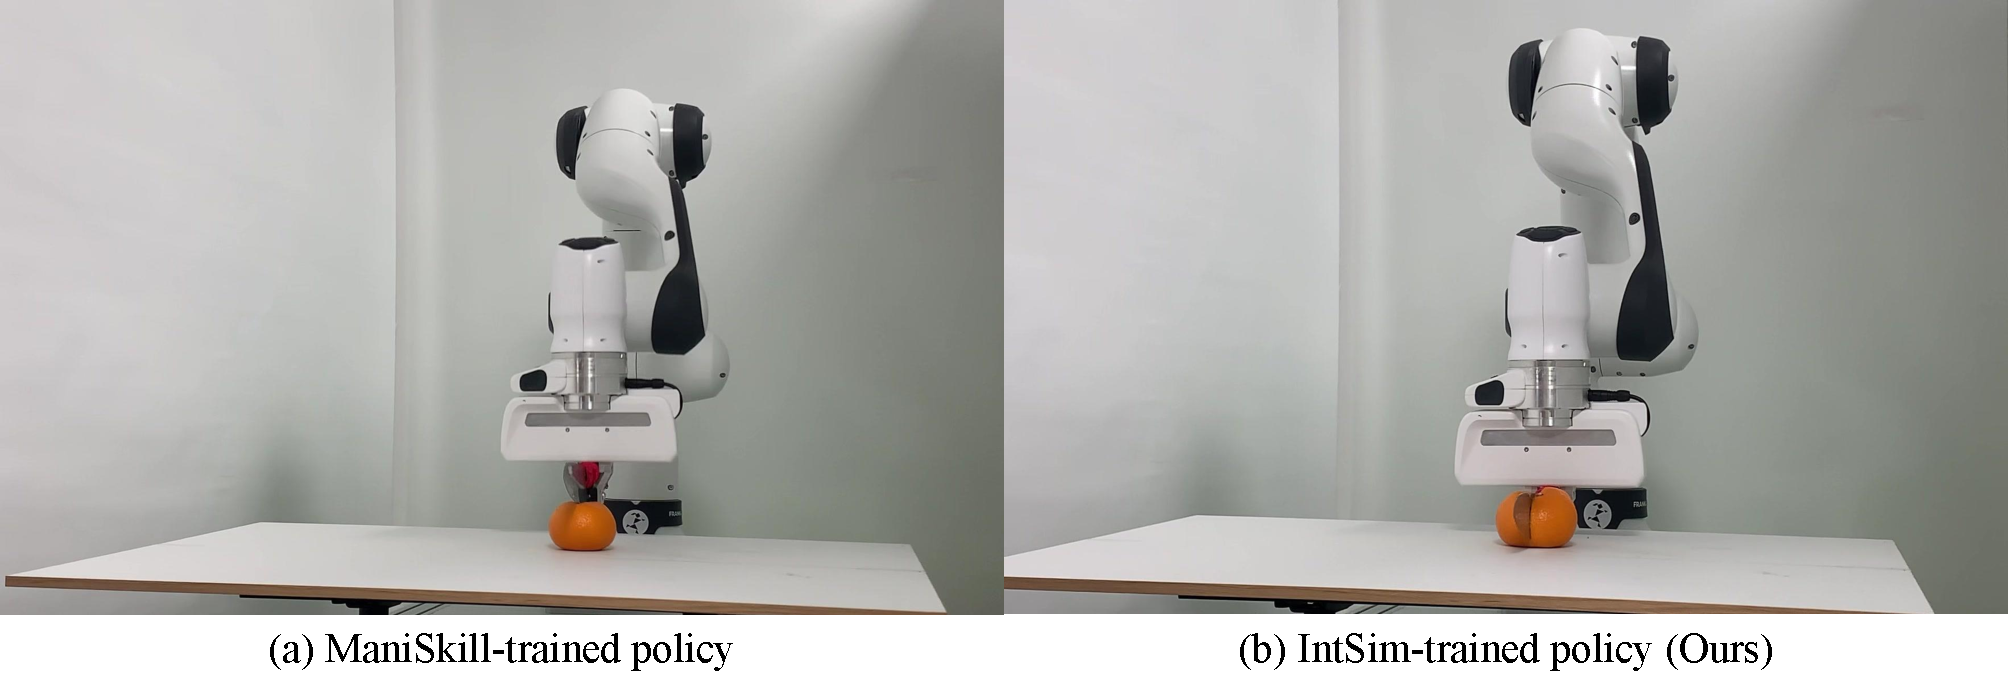
\includegraphics[width=0.88\linewidth]{figure/normal action force-aware action.pdf}
  \caption[{Real-world comparison of trajectory sources}]{\textbf{Real-world comparison of trajectory sources.} Representative Franka Panda orange-cutting attempts contrast a policy fine-tuned on ManiSkill-generated trajectories and one fine-tuned on IntSim-generated physically grounded trajectories. These qualitative examples complement the reported trial-level success rates.}
  \label{fig:cut_real_action_comparison}
\end{figure}

\begin{figure}[!htbp]
  \centering
  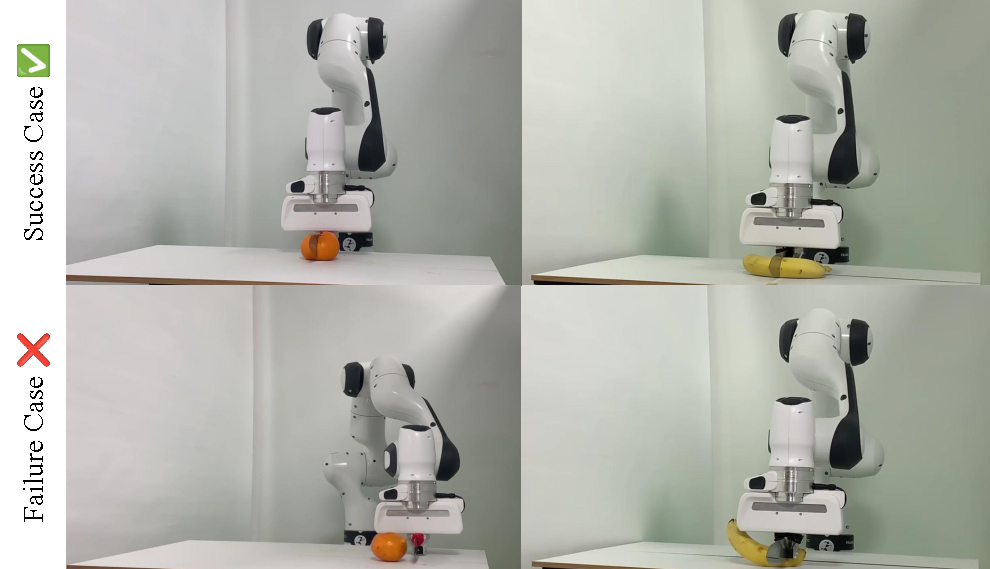
\includegraphics[width=0.90\linewidth]{figure/Real world deployment.pdf}
  \caption[{Real-world orange cutting}]{\textbf{Real-world orange cutting.} Qualitative examples compare RDT fine-tuned using kinematic ManiSkill demonstrations and RDT fine-tuned using IntSim demonstrations. The latter yields more physically effective cutting in the illustrated trials; quantitative results are reported in Table~\ref{tab:cut_physics_gap}.}
  \label{fig:cut_real_deployment}
\end{figure}

\FloatBarrier

\subsection{Ablation: Importance of Topology Updates}
\label{subsec:cut_ablation_topology}

To examine whether the representation of cutting-state changes affects learned behavior, we independently enable or disable post-cut mesh-connectivity updates in training and evaluation. Table~\ref{tab:cut_topology_ablation} reports the resulting RDT success rates. The aligned topology-aware setting achieves 60\%, compared with 55\% when neither training nor evaluation updates topology; mismatched settings decrease to 50\% and 45\%. Beyond these moderate numerical differences, qualitative rollouts reveal that topology-aware training combined with topology-unaware evaluation can cause the policy to repeat a cut, because the observation does not clearly indicate that the previous cut has completed.

\begin{table}[!htbp]
  \centering
  \caption[{RDT topology-update ablation}]{\textbf{RDT topology-update ablation.} ``Yes'' indicates that the object's rendered connectivity is updated after successful cutting.}
  \label{tab:cut_topology_ablation}
  \begingroup
  \CutTableSetup
  \begin{tabularx}{\linewidth}{@{}>{\raggedright\arraybackslash}p{0.27\linewidth}*{3}{>{\centering\arraybackslash}X}@{}}
    \toprule
    Case & Training update & Evaluation update & Success \\
    \midrule
    1 & No & No & 55\% \\
    2 & No & Yes & 50\% \\
    3 & Yes & No & 45\% \\
    4 (ours) & Yes & Yes & \textbf{60\%} \\
    \bottomrule
  \end{tabularx}
  \endgroup
\end{table}

\begin{figure}[!htbp]
  \centering
  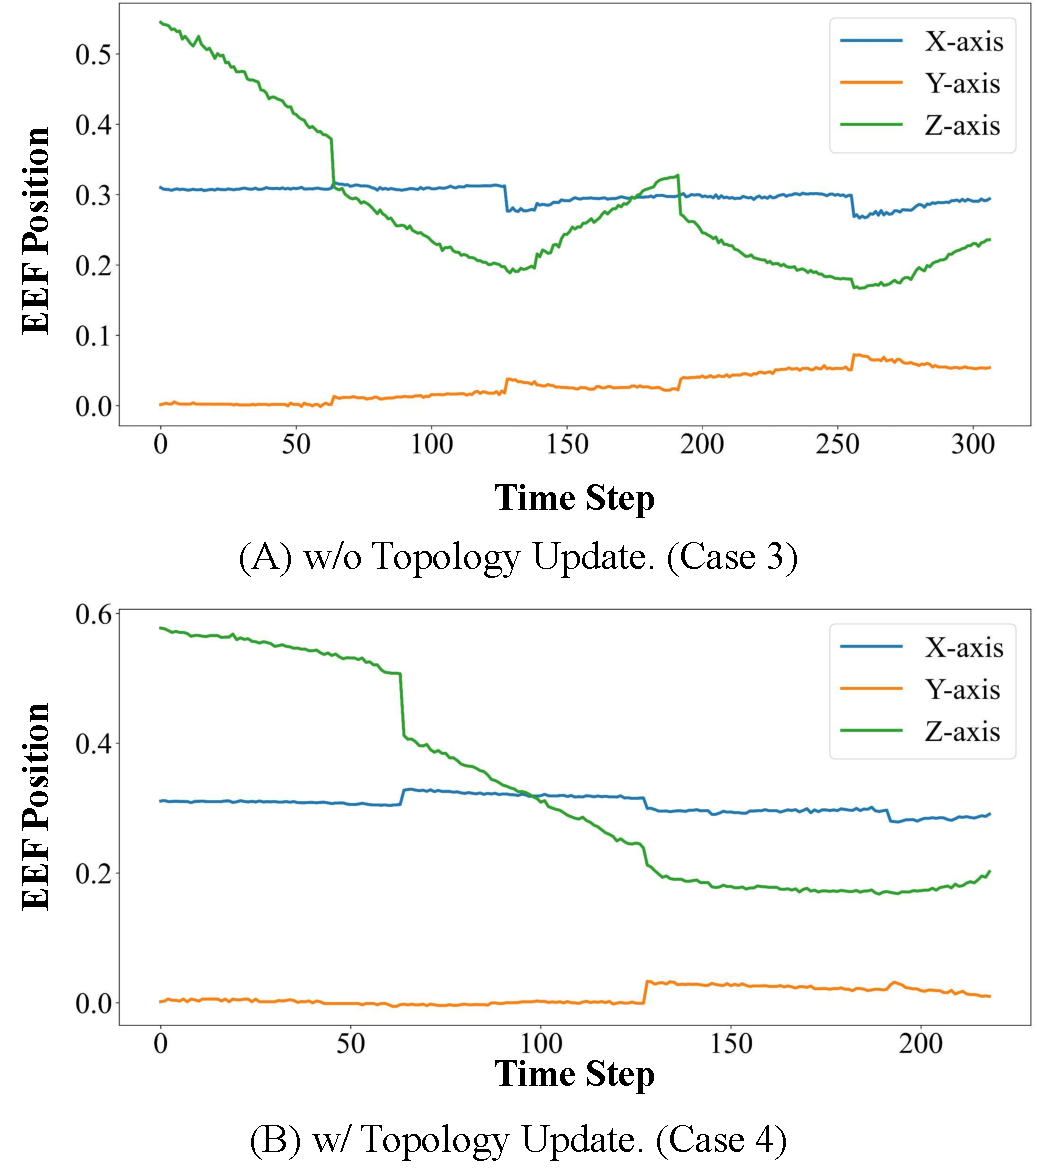
\includegraphics[width=0.82\linewidth]{figure/Supple_ablation_topology.pdf}
  \caption[{Qualitative impact of topology updates}]{\textbf{Qualitative impact of topology updates.} RDT trajectories can revisit an already cut location when post-cut connectivity is not reflected in visual observations; topology-aware evaluation more clearly signals that the cut has completed.}
  \label{fig:cut_topology_effect}
\end{figure}

This finding is consistent with the split-cut results: sequential manipulation requires a representation of \emph{what has already changed}, not simply a memorized knife motion. The ablation does not imply that mesh-connectivity updates alone solve long-horizon planning, since split-cut performance remains poor.

\FloatBarrier

\subsection{Ablation: Execution-Time Velocity Guardrail}
\label{subsec:cut_ablation_guardrail}

The velocity-guardrail ablation uses 20 trials to compare unconstrained execution to filtered end-effector velocities. Without filtering, the reported maximum cutting speed is 3.63\,m/s and maximum contact force reaches 129.31\,N. With the filter enabled, these quantities decrease to 0.89\,m/s and 37.78\,N, respectively. Under the 100\,N threshold used in the study, the unconstrained run exhibits excessive interaction forces, whereas the filtered run suppresses them. These measurements characterize an \emph{external safety mechanism}, not an ablation of force inputs to the learned VLA.

\begin{table}[!htbp]
  \centering
  \caption[{Velocity-guardrail ablation}]{\textbf{Velocity-guardrail ablation.} Reported maximum cutting speed and contact force with and without the execution-time filter.}
  \label{tab:cut_guardrail_ablation}
  \begingroup
  \CutTableSetup
  \begin{tabularx}{\linewidth}{@{}>{\raggedright\arraybackslash}p{0.45\linewidth}*{2}{>{\centering\arraybackslash}X}@{}}
    \toprule
    Execution setting & Max. knife speed & Max. contact force \\
    \midrule
    No guardrail & 3.63\,m/s & 129.31\,N \\
    With guardrail & 0.89\,m/s & 37.78\,N \\
    \bottomrule
  \end{tabularx}
  \endgroup
\end{table}

\begin{figure}[!htbp]
  \centering
  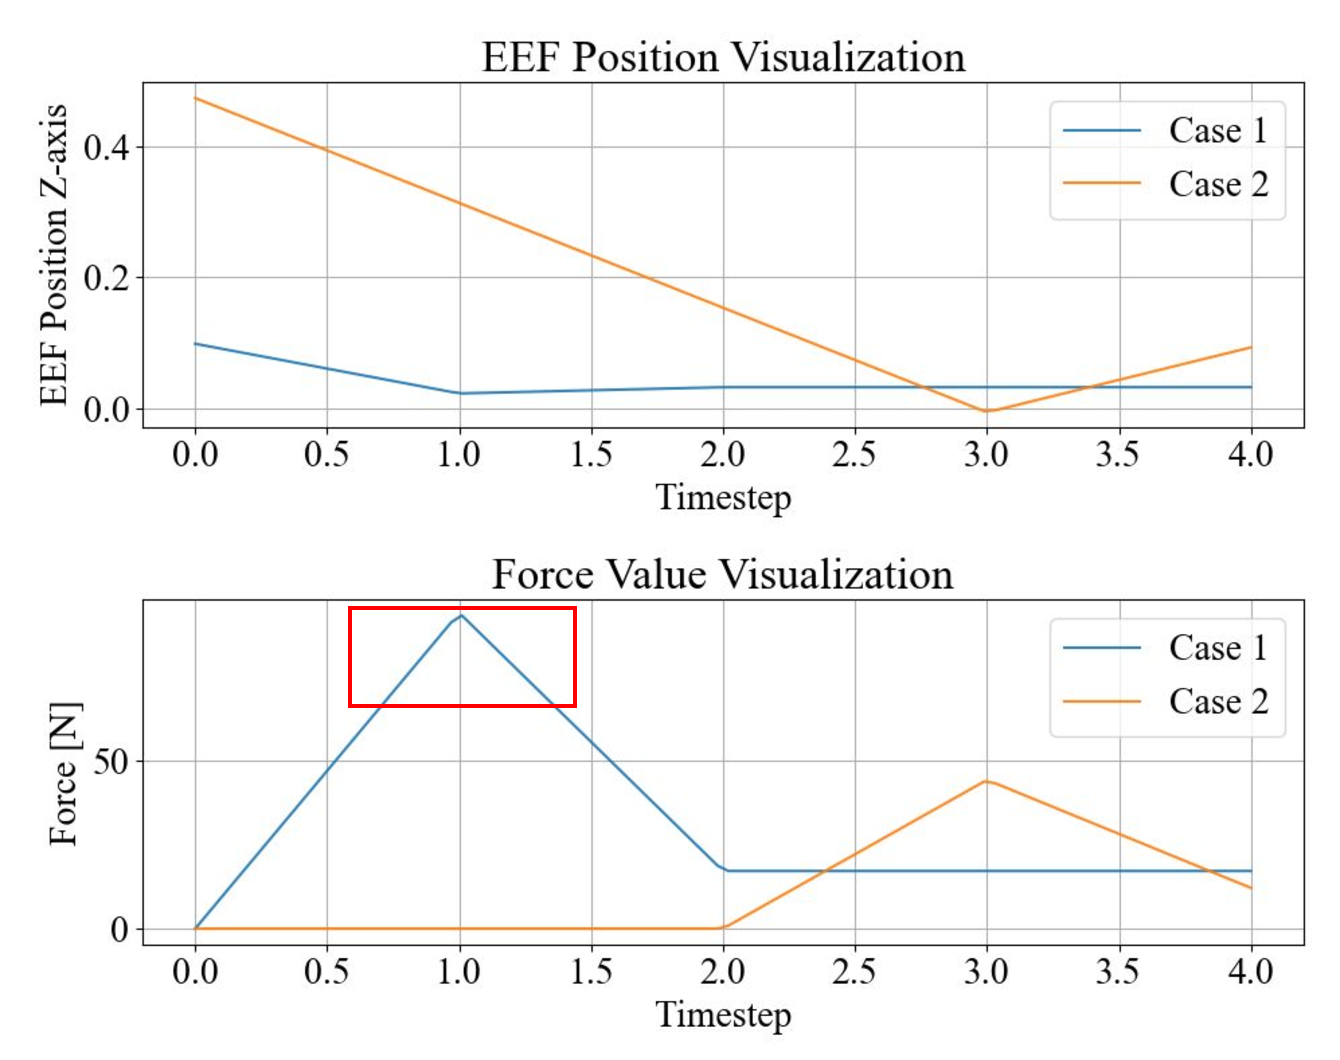
\includegraphics[width=0.83\linewidth]{figure/Figure_sup3.pdf}
  \caption[{Cutting motion and force with the velocity guardrail}]{\textbf{Cutting motion and force with the velocity guardrail.} The evaluation compares vertical end-effector motion and contact-force traces with and without the external velocity clip, illustrating the suppression of sharp force spikes.}
  \label{fig:cut_guardrail_force}
\end{figure}

\FloatBarrier

\subsection{Ablation: Food--Board Friction}
\label{subsec:cut_ablation_friction}

A single-arm cutting arrangement relies on the interaction between the food and cutting board to keep the food from moving with the blade. We compare board--food friction under otherwise matched cutting motions: with board--food friction coefficient $\mu=0.5$, the object is more stable, whereas setting $\mu=0$ yields approximately $0.034$\,m of center-of-mass drift. This effect is important because an object translation can change both the realized ratio location and the contact forces, even if the robot's commanded knife path is unchanged.

\FloatBarrier

\section{Discussion and Limitations}
\label{sec:cut_discussion}

\subsection{Interpreting the Geometry and Physics Gaps}
Object variation, clutter, ratios, and split cuts evaluate how a VLA grounds instructions in geometry. In contrast, the ManiSkill/IntSim comparison assesses whether a geometrically plausible motion actually severs deformable material. The two success criteria are complementary and should not be conflated.

\subsection{What the Benchmark Demonstrates about Simulation}
MLS-MPM provides evolving material states, while signed-distance contact, friction, and damage connect tool motion to deformation and separation. The galleries demonstrate qualitative breadth, whereas measured banana force curves provide narrower quantitative evidence. Improved IntSim-trained RDT performance supports \emph{data-level physical grounding}; it does not establish that the policy learned online force control or an explicit constitutive model.

\subsection{Limitations and Future Directions}
\paragraph*{Material Modeling and Cutting Fidelity}
The material solver approximates cutting using fixed corotated elasticity, optional plasticity, damage-dependent stiffness reduction, and contact rules. It does not explicitly reproduce every relevant tissue fiber, moisture effect, adhesion response, viscoelastic relaxation mechanism, or microscopic fracture process. Its particle--grid discretization can also smooth sharp force transitions. Consequently, the demonstrated resemblance between real and simulated banana force profiles should not be interpreted as complete constitutive validation of fifteen food categories. The reported material parameters are literature-informed starting values with numerical adjustments where needed.

\paragraph*{Scope and Size of Physical Validation}
Force validation focuses on banana cutting, and the real orange-cutting comparison uses ten trials per policy. Broader food categories, cutting styles, and trial counts are required to characterize physical fidelity and deployment uncertainty.

\paragraph*{Object Stabilization and Execution}
Single-arm cutting relies on passive friction against the board. Its removal produces centimeter-scale drift in the reported ablation; active holding and its additional contact mechanics remain future work.

\paragraph*{Visual Realism and World-Model Augmentation}
The simulator's images retain a real-world appearance gap. We also examine Cosmos-based appearance enhancement~\citep{nvidia2025cosmosworldfoundationmodel} while preserving the underlying cutting sequence. Such enhancement complements physical modeling but does not improve force or fracture accuracy by itself (Figure~\ref{fig:cut_world_model}).

\begin{figure}[!htbp]
  \centering
  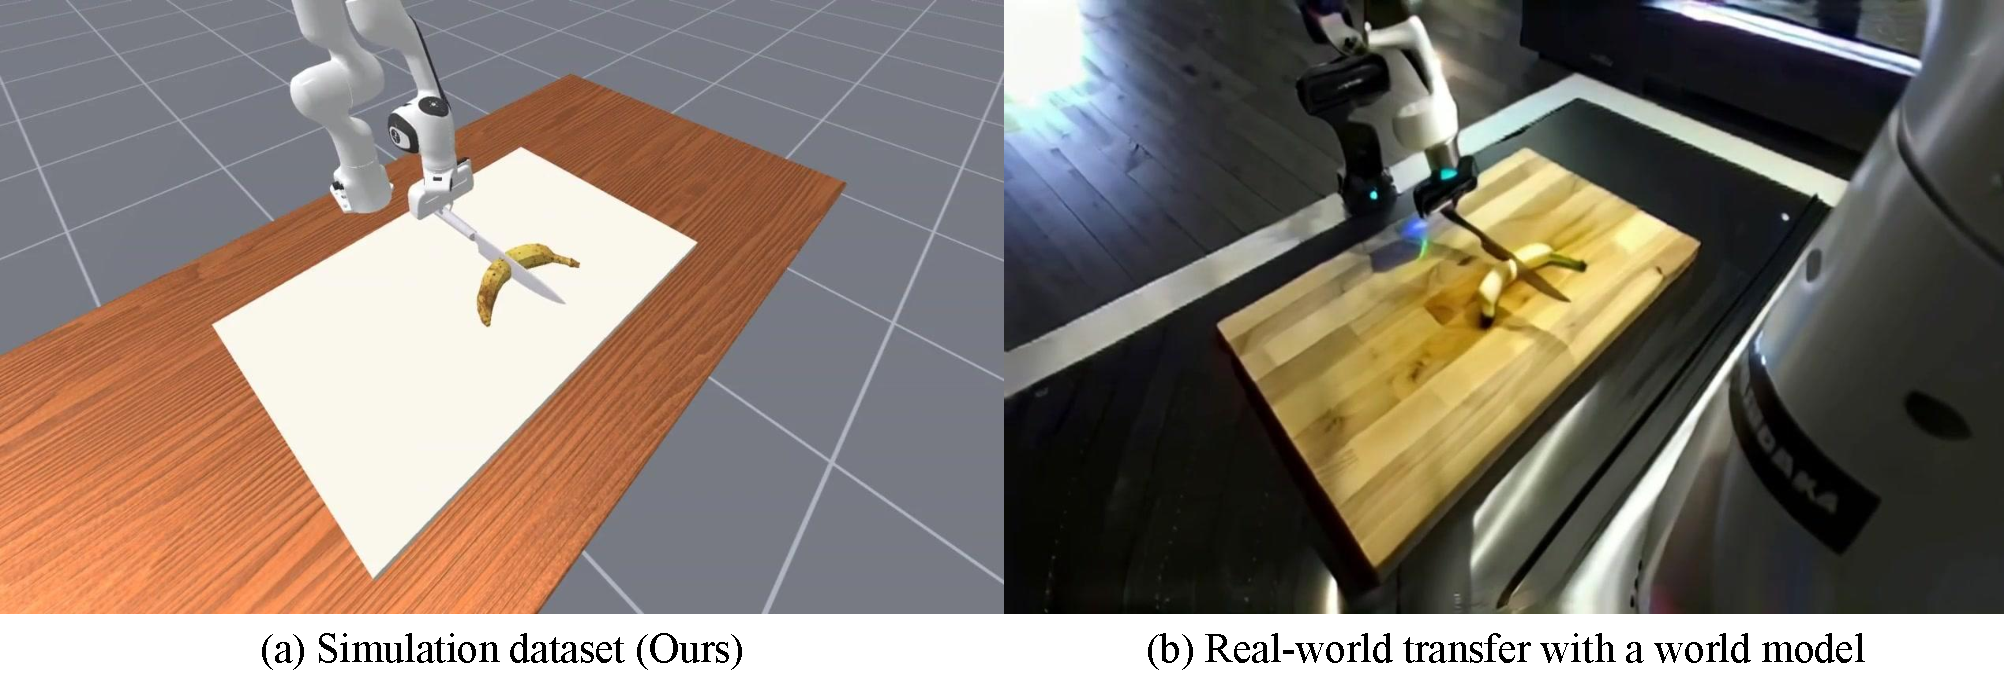
\includegraphics[width=\linewidth]{figure/world model.pdf}
  \caption[{Exploratory visual enhancement with Cosmos}]{\textbf{Exploratory visual enhancement with Cosmos.} The figure compares simulator-rendered cutting frames with appearance-enhanced outputs. Visual enhancement is complementary to, not a replacement for, the physical simulation and force validation in IntSim.}
  \label{fig:cut_world_model}
\end{figure}

\FloatBarrier

\section{Chapter Summary}
\label{sec:cut_summary}

This chapter introduced CulinaryCut and its IntSim environment, which couples MLS-MPM deformable dynamics to ManiSkill robot execution. The solver uses fixed corotated elasticity, optional plasticity, damage, tool contact, and numerical safeguards to generate and evaluate cutting trajectories beyond geometric knife placement.

CulinaryCut comprises 21,000 base trajectories over 15 foods, augmented to approximately 1.575 million instances. VLA experiments reveal both geometry and physics gaps. With unchanged RDT architecture and force-free inference, IntSim-grounded training improves physical orange-cutting success from 23\% to 59\% in integrated simulation, with an initial real-robot improvement from 1/10 to 3/10. These findings support physics-grounded simulation as a source of richer data and more meaningful evaluation for deformable manipulation.

\FloatBarrier
